\documentclass[1p]{elsarticle_modified}
%\bibliographystyle{elsarticle-num}

%\usepackage[colorlinks]{hyperref}
%\usepackage{abbrmath_seonhwa} %\Abb, \Ascr, \Acal ,\Abf, \Afrak
\usepackage{amsfonts}
\usepackage{amssymb}
\usepackage{amsmath}
\usepackage{amsthm}
\usepackage{scalefnt}
\usepackage{amsbsy}
\usepackage{kotex}
\usepackage{caption}
\usepackage{subfig}
\usepackage{color}
\usepackage{graphicx}
\usepackage{xcolor} %% white, black, red, green, blue, cyan, magenta, yellow
\usepackage{float}
\usepackage{setspace}
\usepackage{hyperref}

\usepackage{tikz}
\usetikzlibrary{arrows}

\usepackage{multirow}
\usepackage{array} % fixed length table
\usepackage{hhline}

%%%%%%%%%%%%%%%%%%%%%
\makeatletter
\renewcommand*\env@matrix[1][\arraystretch]{%
	\edef\arraystretch{#1}%
	\hskip -\arraycolsep
	\let\@ifnextchar\new@ifnextchar
	\array{*\c@MaxMatrixCols c}}
\makeatother %https://tex.stackexchange.com/questions/14071/how-can-i-increase-the-line-spacing-in-a-matrix
%%%%%%%%%%%%%%%

\usepackage[normalem]{ulem}

\newcommand{\msout}[1]{\ifmmode\text{\sout{\ensuremath{#1}}}\else\sout{#1}\fi}
%SOURCE: \msout is \stkout macro in https://tex.stackexchange.com/questions/20609/strikeout-in-math-mode

\newcommand{\cancel}[1]{
	\ifmmode
	{\color{red}\msout{#1}}
	\else
	{\color{red}\sout{#1}}
	\fi
}

\newcommand{\add}[1]{
	{\color{blue}\uwave{#1}}
}

\newcommand{\replace}[2]{
	\ifmmode
	{\color{red}\msout{#1}}{\color{blue}\uwave{#2}}
	\else
	{\color{red}\sout{#1}}{\color{blue}\uwave{#2}}
	\fi
}

\newcommand{\Sol}{\mathcal{S}} %segment
\newcommand{\D}{D} %diagram
\newcommand{\A}{\mathcal{A}} %arc


%%%%%%%%%%%%%%%%%%%%%%%%%%%%%5 test

\def\sl{\operatorname{\textup{SL}}(2,\Cbb)}
\def\psl{\operatorname{\textup{PSL}}(2,\Cbb)}
\def\quan{\mkern 1mu \triangleright \mkern 1mu}

\theoremstyle{definition}
\newtheorem{thm}{Theorem}[section]
\newtheorem{prop}[thm]{Proposition}
\newtheorem{lem}[thm]{Lemma}
\newtheorem{ques}[thm]{Question}
\newtheorem{cor}[thm]{Corollary}
\newtheorem{defn}[thm]{Definition}
\newtheorem{exam}[thm]{Example}
\newtheorem{rmk}[thm]{Remark}
\newtheorem{alg}[thm]{Algorithm}

\newcommand{\I}{\sqrt{-1}}
\begin{document}

%\begin{frontmatter}
%
%\title{Boundary parabolic representations of knots up to 8 crossings}
%
%%% Group authors per affiliation:
%\author{Yunhi Cho} 
%\address{Department of Mathematics, University of Seoul, Seoul, Korea}
%\ead{yhcho@uos.ac.kr}
%
%
%\author{Seonhwa Kim} %\fnref{s_kim}}
%\address{Center for Geometry and Physics, Institute for Basic Science, Pohang, 37673, Korea}
%\ead{ryeona17@ibs.re.kr}
%
%\author{Hyuk Kim}
%\address{Department of Mathematical Sciences, Seoul National University, Seoul 08826, Korea}
%\ead{hyukkim@snu.ac.kr}
%
%\author{Seokbeom Yoon}
%\address{Department of Mathematical Sciences, Seoul National University, Seoul, 08826,  Korea}
%\ead{sbyoon15@snu.ac.kr}
%
%\begin{abstract}
%We find all boundary parabolic representation of knots up to 8 crossings.
%
%\end{abstract}
%\begin{keyword}
%    \MSC[2010] 57M25 
%\end{keyword}
%
%\end{frontmatter}

%\linenumbers
%\tableofcontents
%
\newcommand\colored[1]{\textcolor{white}{\rule[-0.35ex]{0.8em}{1.4ex}}\kern-0.8em\color{red} #1}%
%\newcommand\colored[1]{\textcolor{white}{ #1}\kern-2.17ex	\textcolor{white}{ #1}\kern-1.81ex	\textcolor{white}{ #1}\kern-2.15ex\color{red}#1	}

{\Large $\underline{12a_{0698}~(K12a_{0698})}$}

\setlength{\tabcolsep}{10pt}
\renewcommand{\arraystretch}{1.6}
\vspace{1cm}\begin{tabular}{m{100pt}>{\centering\arraybackslash}m{274pt}}
\multirow{5}{120pt}{
	\centering
	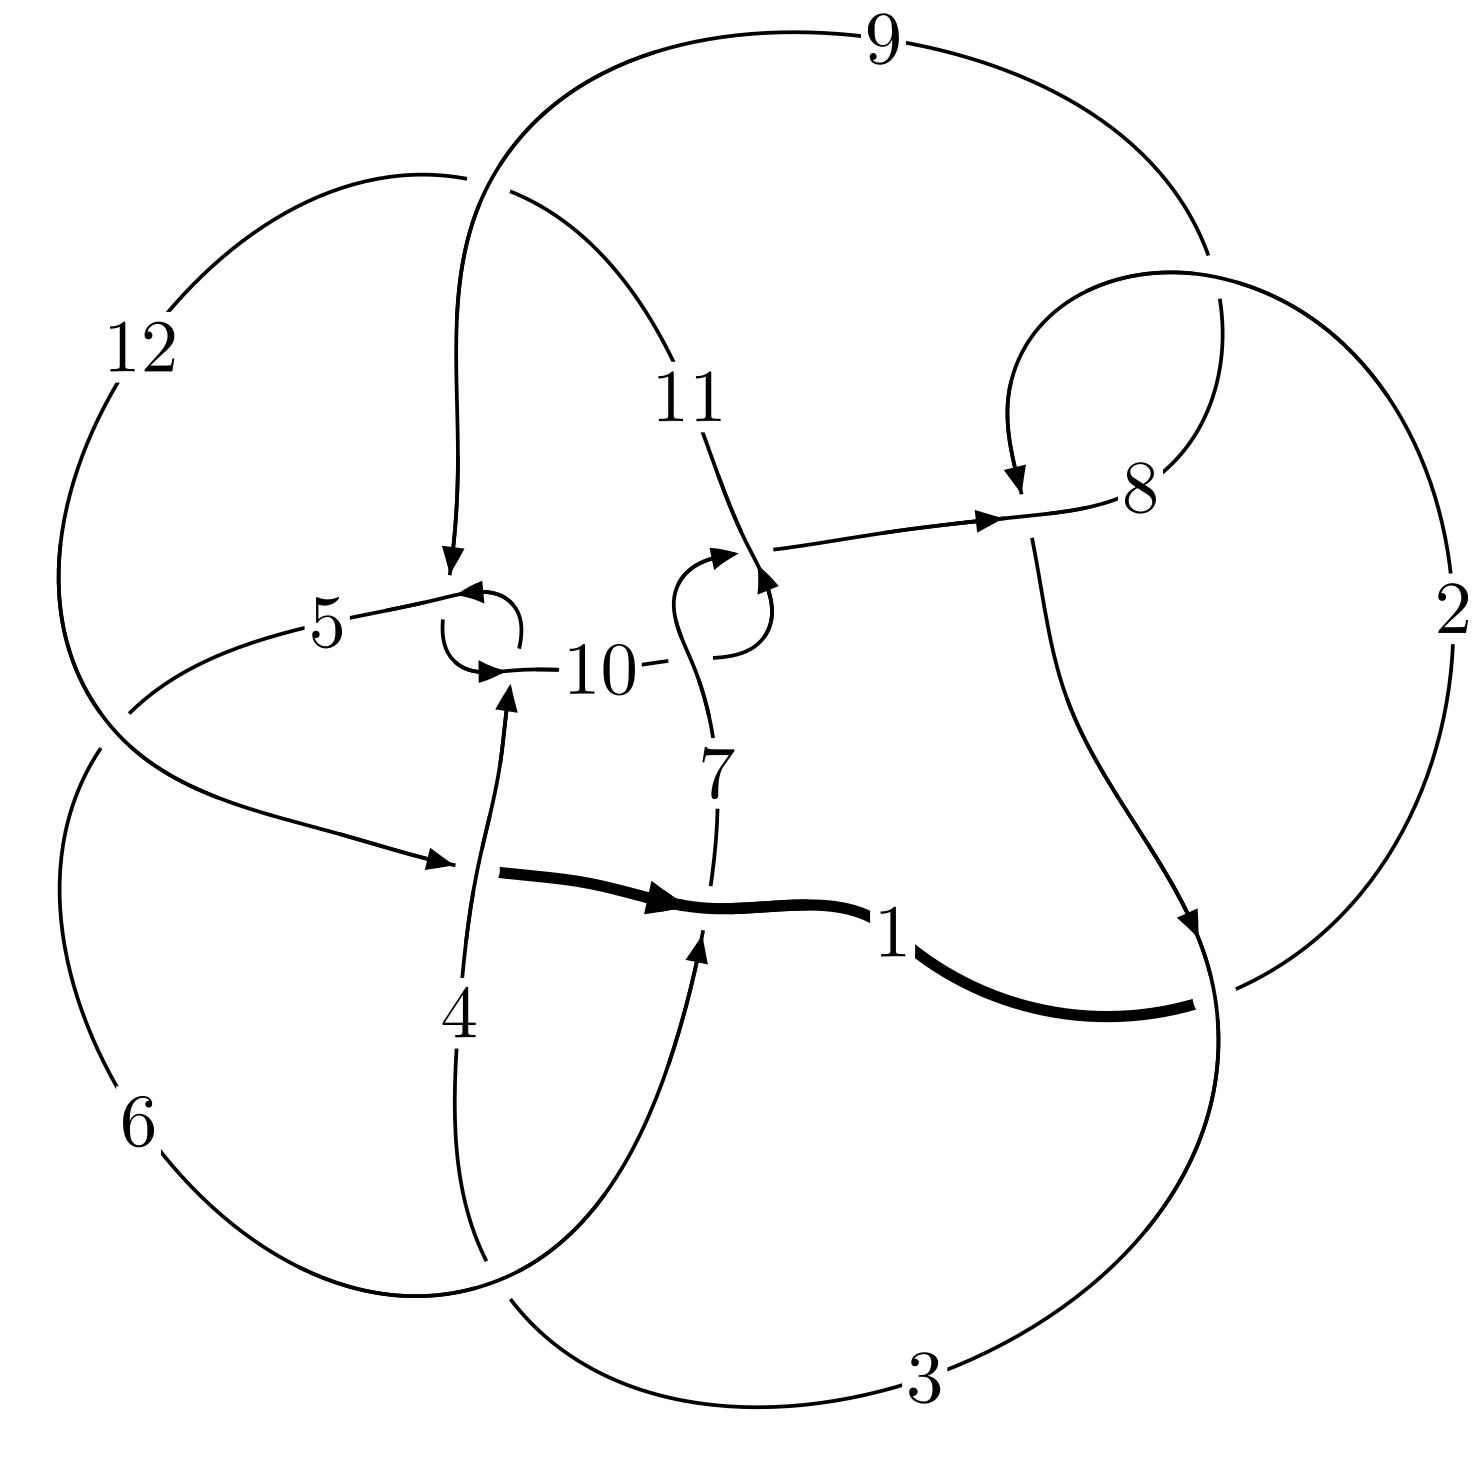
\includegraphics[width=112pt]{../../../GIT/diagram.site/Diagrams/png/1499_12a_0698.png}\\
\ \ \ A knot diagram\footnotemark}&
\allowdisplaybreaks
\textbf{Linearized knot diagam} \\
\cline{2-2}
 &
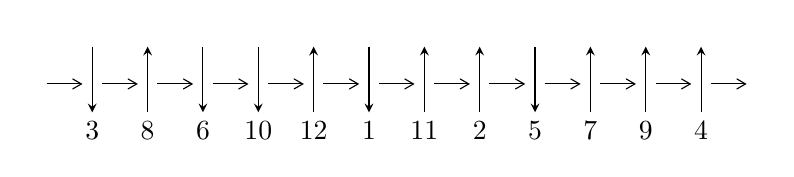
\begin{tikzpicture}[x=20pt, y=17pt]
	% nodes
	\node (C0) at (0, 0) {};
	\node (C1) at (1, 0) {};
	\node (C1U) at (1, +1) {};
	\node (C1D) at (1, -1) {3};

	\node (C2) at (2, 0) {};
	\node (C2U) at (2, +1) {};
	\node (C2D) at (2, -1) {8};

	\node (C3) at (3, 0) {};
	\node (C3U) at (3, +1) {};
	\node (C3D) at (3, -1) {6};

	\node (C4) at (4, 0) {};
	\node (C4U) at (4, +1) {};
	\node (C4D) at (4, -1) {10};

	\node (C5) at (5, 0) {};
	\node (C5U) at (5, +1) {};
	\node (C5D) at (5, -1) {12};

	\node (C6) at (6, 0) {};
	\node (C6U) at (6, +1) {};
	\node (C6D) at (6, -1) {1};

	\node (C7) at (7, 0) {};
	\node (C7U) at (7, +1) {};
	\node (C7D) at (7, -1) {11};

	\node (C8) at (8, 0) {};
	\node (C8U) at (8, +1) {};
	\node (C8D) at (8, -1) {2};

	\node (C9) at (9, 0) {};
	\node (C9U) at (9, +1) {};
	\node (C9D) at (9, -1) {5};

	\node (C10) at (10, 0) {};
	\node (C10U) at (10, +1) {};
	\node (C10D) at (10, -1) {7};

	\node (C11) at (11, 0) {};
	\node (C11U) at (11, +1) {};
	\node (C11D) at (11, -1) {9};

	\node (C12) at (12, 0) {};
	\node (C12U) at (12, +1) {};
	\node (C12D) at (12, -1) {4};
	\node (C13) at (13, 0) {};

	% arrows
	\draw[->,>={angle 60}]
	(C0) edge (C1) (C1) edge (C2) (C2) edge (C3) (C3) edge (C4) (C4) edge (C5) (C5) edge (C6) (C6) edge (C7) (C7) edge (C8) (C8) edge (C9) (C9) edge (C10) (C10) edge (C11) (C11) edge (C12) (C12) edge (C13) ;	\draw[->,>=stealth]
	(C1U) edge (C1D) (C2D) edge (C2U) (C3U) edge (C3D) (C4U) edge (C4D) (C5D) edge (C5U) (C6U) edge (C6D) (C7D) edge (C7U) (C8D) edge (C8U) (C9U) edge (C9D) (C10D) edge (C10U) (C11D) edge (C11U) (C12D) edge (C12U) ;
	\end{tikzpicture} \\
\hhline{~~} \\& 
\textbf{Solving Sequence} \\ \cline{2-2} 
 &
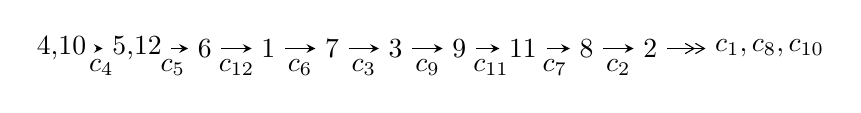
\begin{tikzpicture}[x=23pt, y=7pt]
	% node
	\node (A0) at (-1/8, 0) {4,10};
	\node (A1) at (17/16, 0) {5,12};
	\node (A2) at (17/8, 0) {6};
	\node (A3) at (25/8, 0) {1};
	\node (A4) at (33/8, 0) {7};
	\node (A5) at (41/8, 0) {3};
	\node (A6) at (49/8, 0) {9};
	\node (A7) at (57/8, 0) {11};
	\node (A8) at (65/8, 0) {8};
	\node (A9) at (73/8, 0) {2};
	\node (C1) at (1/2, -1) {$c_{4}$};
	\node (C2) at (13/8, -1) {$c_{5}$};
	\node (C3) at (21/8, -1) {$c_{12}$};
	\node (C4) at (29/8, -1) {$c_{6}$};
	\node (C5) at (37/8, -1) {$c_{3}$};
	\node (C6) at (45/8, -1) {$c_{9}$};
	\node (C7) at (53/8, -1) {$c_{11}$};
	\node (C8) at (61/8, -1) {$c_{7}$};
	\node (C9) at (69/8, -1) {$c_{2}$};
	\node (A10) at (11, 0) {$c_{1},c_{8},c_{10}$};

	% edge
	\draw[->,>=stealth]	
	(A0) edge (A1) (A1) edge (A2) (A2) edge (A3) (A3) edge (A4) (A4) edge (A5) (A5) edge (A6) (A6) edge (A7) (A7) edge (A8) (A8) edge (A9) ;
	\draw[->>,>={angle 60}]	
	(A9) edge (A10);
\end{tikzpicture} \\ 

\end{tabular} \\

\footnotetext{
The image of knot diagram is generated by the software ``\textbf{Draw programme}" developed by Andrew Bartholomew(\url{http://www.layer8.co.uk/maths/draw/index.htm\#Running-draw}), where we modified some parts for our purpose(\url{https://github.com/CATsTAILs/LinksPainter}).
}\phantom \\ \newline 
\centering \textbf{Ideals for irreducible components\footnotemark of $X_{\text{par}}$} 
 
\begin{align*}
I^u_{1}&=\langle 
-5.93801\times10^{1004} u^{165}-6.10876\times10^{1004} u^{164}+\cdots+4.43418\times10^{1003} b+4.56960\times10^{1008},\\
\phantom{I^u_{1}}&\phantom{= \langle  }1.93137\times10^{1009} u^{165}+1.57216\times10^{1009} u^{164}+\cdots+1.53746\times10^{1008} a-9.46926\times10^{1012},\\
\phantom{I^u_{1}}&\phantom{= \langle  }3 u^{166}+u^{165}+\cdots+158795 u-34673\rangle \\
I^u_{2}&=\langle 
-3.22786\times10^{28} u^{40}-2.94202\times10^{28} u^{39}+\cdots+7.20126\times10^{23} b+7.42965\times10^{27},\\
\phantom{I^u_{2}}&\phantom{= \langle  }2.04412\times10^{29} u^{40}+2.34054\times10^{29} u^{39}+\cdots+7.20126\times10^{23} a-2.07039\times10^{28},\;3 u^{41}+4 u^{40}+\cdots-2 u+1\rangle \\
\\
\end{align*}
\raggedright * 2 irreducible components of $\dim_{\mathbb{C}}=0$, with total 207 representations.\\
\footnotetext{All coefficients of polynomials are rational numbers. But the coefficients are sometimes approximated in decimal forms when there is not enough margin.}
\newpage
\renewcommand{\arraystretch}{1}
\centering \section*{I. $I^u_{1}= \langle -5.94\times10^{1004} u^{165}-6.11\times10^{1004} u^{164}+\cdots+4.43\times10^{1003} b+4.57\times10^{1008},\;1.93\times10^{1009} u^{165}+1.57\times10^{1009} u^{164}+\cdots+1.54\times10^{1008} a-9.47\times10^{1012},\;3 u^{166}+u^{165}+\cdots+158795 u-34673 \rangle$}
\flushleft \textbf{(i) Arc colorings}\\
\begin{tabular}{m{7pt} m{180pt} m{7pt} m{180pt} }
\flushright $a_{4}=$&$\begin{pmatrix}1\\0\end{pmatrix}$ \\
\flushright $a_{10}=$&$\begin{pmatrix}0\\u\end{pmatrix}$ \\
\flushright $a_{5}=$&$\begin{pmatrix}1\\u^2\end{pmatrix}$ \\
\flushright $a_{12}=$&$\begin{pmatrix}-12.5620 u^{165}-10.2257 u^{164}+\cdots-115249. u+61590.1\\13.3914 u^{165}+13.7765 u^{164}+\cdots+297471. u-103054.\end{pmatrix}$ \\
\flushright $a_{6}=$&$\begin{pmatrix}4.50111 u^{165}+9.08946 u^{164}+\cdots+312445. u-81523.8\\4.18966 u^{165}-1.18288 u^{164}+\cdots-208987. u+35460.0\end{pmatrix}$ \\
\flushright $a_{1}=$&$\begin{pmatrix}0.829406 u^{165}+3.55083 u^{164}+\cdots+182221. u-41463.9\\13.3914 u^{165}+13.7765 u^{164}+\cdots+297471. u-103054.\end{pmatrix}$ \\
\flushright $a_{7}=$&$\begin{pmatrix}8.10917 u^{165}+8.55775 u^{164}+\cdots+182756. u-62856.9\\1.44500 u^{165}+2.27183 u^{164}+\cdots+100018. u-24448.9\end{pmatrix}$ \\
\flushright $a_{3}=$&$\begin{pmatrix}3.72196 u^{165}-8.01983 u^{164}+\cdots-578450. u+117911.\\-6.77876 u^{165}-8.62088 u^{164}+\cdots-238138. u+71425.4\end{pmatrix}$ \\
\flushright $a_{9}=$&$\begin{pmatrix}u\\u^3+u\end{pmatrix}$ \\
\flushright $a_{11}=$&$\begin{pmatrix}0.840773 u^{165}+3.51002 u^{164}+\cdots+177388. u-40546.1\\15.0557 u^{165}+14.0762 u^{164}+\cdots+254436. u-98072.5\end{pmatrix}$ \\
\flushright $a_{8}=$&$\begin{pmatrix}6.77989 u^{165}+11.7779 u^{164}+\cdots+387456. u-104685.\\5.30148 u^{165}-2.53704 u^{164}+\cdots-323400. u+58111.5\end{pmatrix}$ \\
\flushright $a_{2}=$&$\begin{pmatrix}-6.11877 u^{165}+0.116900 u^{164}+\cdots+211422. u-31703.0\\2.04072 u^{165}+3.41291 u^{164}+\cdots+108062. u-29669.1\end{pmatrix}$\\&\end{tabular}
\flushleft \textbf{(ii) Obstruction class $= -1$}\\~\\
\flushleft \textbf{(iii) Cusp Shapes $= 4.35284 u^{165}+5.59579 u^{164}+\cdots+185940. u-52310.4$}\\~\\
\newpage\renewcommand{\arraystretch}{1}
\flushleft \textbf{(iv) u-Polynomials at the component}\newline \\
\begin{tabular}{m{50pt}|m{274pt}}
Crossings & \hspace{64pt}u-Polynomials at each crossing \\
\hline $$\begin{aligned}c_{1}\end{aligned}$$&$\begin{aligned}
&9(9 u^{166}+548 u^{165}+\cdots+1674688 u+37249)
\end{aligned}$\\
\hline $$\begin{aligned}c_{2},c_{8}\end{aligned}$$&$\begin{aligned}
&3(3 u^{166}+10 u^{165}+\cdots-72 u-193)
\end{aligned}$\\
\hline $$\begin{aligned}c_{3}\end{aligned}$$&$\begin{aligned}
&u^{166}-26 u^{165}+\cdots-3326078 u+219087
\end{aligned}$\\
\hline $$\begin{aligned}c_{4},c_{9}\end{aligned}$$&$\begin{aligned}
&3(3 u^{166}+u^{165}+\cdots+158795 u-34673)
\end{aligned}$\\
\hline $$\begin{aligned}c_{5}\end{aligned}$$&$\begin{aligned}
&u^{166}+u^{165}+\cdots+3422516 u-262817
\end{aligned}$\\
\hline $$\begin{aligned}c_{6}\end{aligned}$$&$\begin{aligned}
&u^{166}+2 u^{165}+\cdots+2824430 u+436239
\end{aligned}$\\
\hline $$\begin{aligned}c_{7},c_{10}\end{aligned}$$&$\begin{aligned}
&u^{166}-49 u^{164}+\cdots+2520956 u+2425663
\end{aligned}$\\
\hline $$\begin{aligned}c_{11}\end{aligned}$$&$\begin{aligned}
&u^{166}+9 u^{165}+\cdots+3480001987 u+3246415791
\end{aligned}$\\
\hline $$\begin{aligned}c_{12}\end{aligned}$$&$\begin{aligned}
&9(9 u^{166}+98 u^{165}+\cdots-12 u-1)
\end{aligned}$\\
\hline
\end{tabular}\\~\\
\newpage\renewcommand{\arraystretch}{1}
\flushleft \textbf{(v) Riley Polynomials at the component}\newline \\
\begin{tabular}{m{50pt}|m{274pt}}
Crossings & \hspace{64pt}Riley Polynomials at each crossing \\
\hline $$\begin{aligned}c_{1}\end{aligned}$$&$\begin{aligned}
&81(81 y^{166}+5408 y^{165}+\cdots-2.42908\times10^{11} y+1.38749\times10^{9})
\end{aligned}$\\
\hline $$\begin{aligned}c_{2},c_{8}\end{aligned}$$&$\begin{aligned}
&9(9 y^{166}+548 y^{165}+\cdots+1674688 y+37249)
\end{aligned}$\\
\hline $$\begin{aligned}c_{3}\end{aligned}$$&$\begin{aligned}
&y^{166}-4 y^{165}+\cdots+1995653540696 y+47999113569
\end{aligned}$\\
\hline $$\begin{aligned}c_{4},c_{9}\end{aligned}$$&$\begin{aligned}
&9(9 y^{166}+1043 y^{165}+\cdots+3.28301\times10^{10} y+1.20222\times10^{9})
\end{aligned}$\\
\hline $$\begin{aligned}c_{5}\end{aligned}$$&$\begin{aligned}
&y^{166}-27 y^{165}+\cdots+21178704987358 y+69072775489
\end{aligned}$\\
\hline $$\begin{aligned}c_{6}\end{aligned}$$&$\begin{aligned}
&y^{166}+34 y^{165}+\cdots+7330681481006 y+190304465121
\end{aligned}$\\
\hline $$\begin{aligned}c_{7},c_{10}\end{aligned}$$&$\begin{aligned}
&y^{166}-98 y^{165}+\cdots+164556690192526 y+5883840989569
\end{aligned}$\\
\hline $$\begin{aligned}c_{11}\end{aligned}$$&$\begin{aligned}
&y^{166}-69 y^{165}+\cdots-4.67\times10^{20} y+1.05\times10^{19}
\end{aligned}$\\
\hline $$\begin{aligned}c_{12}\end{aligned}$$&$\begin{aligned}
&81(81 y^{166}-2044 y^{165}+\cdots+118 y+1)
\end{aligned}$\\
\hline
\end{tabular}\\~\\
\newpage\flushleft \textbf{(vi) Complex Volumes and Cusp Shapes}
$$\begin{array}{c|c|c}  
\text{Solutions to }I^u_{1}& \I (\text{vol} + \sqrt{-1}CS) & \text{Cusp shape}\\
 \hline 
\begin{aligned}
u &= -0.448185 + 0.894932 I \\
a &= \phantom{-}2.49663 - 0.47452 I \\
b &= -1.38436 - 0.77923 I\end{aligned}
 & \phantom{-}2.42095 + 10.29690 I & \phantom{-0.000000 } 0 \\ \hline\begin{aligned}
u &= -0.448185 - 0.894932 I \\
a &= \phantom{-}2.49663 + 0.47452 I \\
b &= -1.38436 + 0.77923 I\end{aligned}
 & \phantom{-}2.42095 - 10.29690 I & \phantom{-0.000000 } 0 \\ \hline\begin{aligned}
u &= -0.242605 + 0.974518 I \\
a &= \phantom{-}2.69617 + 0.37041 I \\
b &= -1.67458 - 1.36534 I\end{aligned}
 & -0.32447 + 3.71499 I & \phantom{-0.000000 } 0 \\ \hline\begin{aligned}
u &= -0.242605 - 0.974518 I \\
a &= \phantom{-}2.69617 - 0.37041 I \\
b &= -1.67458 + 1.36534 I\end{aligned}
 & -0.32447 - 3.71499 I & \phantom{-0.000000 } 0 \\ \hline\begin{aligned}
u &= \phantom{-}0.029029 + 0.990881 I \\
a &= \phantom{-}0.09091 + 1.85495 I \\
b &= -0.014668 + 0.843715 I\end{aligned}
 & -0.16410 - 2.59463 I & \phantom{-0.000000 } 0 \\ \hline\begin{aligned}
u &= \phantom{-}0.029029 - 0.990881 I \\
a &= \phantom{-}0.09091 - 1.85495 I \\
b &= -0.014668 - 0.843715 I\end{aligned}
 & -0.16410 + 2.59463 I & \phantom{-0.000000 } 0 \\ \hline\begin{aligned}
u &= \phantom{-}0.082464 + 0.984904 I \\
a &= -0.1156355 + 0.0157277 I \\
b &= \phantom{-}0.304104 - 1.321090 I\end{aligned}
 & \phantom{-}2.53184 - 2.60316 I & \phantom{-0.000000 } 0 \\ \hline\begin{aligned}
u &= \phantom{-}0.082464 - 0.984904 I \\
a &= -0.1156355 - 0.0157277 I \\
b &= \phantom{-}0.304104 + 1.321090 I\end{aligned}
 & \phantom{-}2.53184 + 2.60316 I & \phantom{-0.000000 } 0 \\ \hline\begin{aligned}
u &= \phantom{-}0.027624 + 0.970485 I \\
a &= \phantom{-}0.038744 + 0.780028 I \\
b &= -0.33961 - 1.73805 I\end{aligned}
 & -1.11542 - 1.19066 I & \phantom{-0.000000 } 0 \\ \hline\begin{aligned}
u &= \phantom{-}0.027624 - 0.970485 I \\
a &= \phantom{-}0.038744 - 0.780028 I \\
b &= -0.33961 + 1.73805 I\end{aligned}
 & -1.11542 + 1.19066 I & \phantom{-0.000000 } 0\\
 \hline 
 \end{array}$$\newpage$$\begin{array}{c|c|c}  
\text{Solutions to }I^u_{1}& \I (\text{vol} + \sqrt{-1}CS) & \text{Cusp shape}\\
 \hline 
\begin{aligned}
u &= -0.620419 + 0.736789 I \\
a &= \phantom{-}0.153850 - 0.200517 I \\
b &= \phantom{-}0.171744 + 0.401489 I\end{aligned}
 & \phantom{-}0.20448 + 1.78532 I & \phantom{-0.000000 } 0 \\ \hline\begin{aligned}
u &= -0.620419 - 0.736789 I \\
a &= \phantom{-}0.153850 + 0.200517 I \\
b &= \phantom{-}0.171744 - 0.401489 I\end{aligned}
 & \phantom{-}0.20448 - 1.78532 I & \phantom{-0.000000 } 0 \\ \hline\begin{aligned}
u &= -0.936987 + 0.205652 I \\
a &= -0.022756 + 0.192563 I \\
b &= -0.662032 + 0.927484 I\end{aligned}
 & -4.24556 - 2.17045 I & \phantom{-0.000000 } 0 \\ \hline\begin{aligned}
u &= -0.936987 - 0.205652 I \\
a &= -0.022756 - 0.192563 I \\
b &= -0.662032 - 0.927484 I\end{aligned}
 & -4.24556 + 2.17045 I & \phantom{-0.000000 } 0 \\ \hline\begin{aligned}
u &= \phantom{-}0.042824 + 0.954124 I \\
a &= \phantom{-}1.97457 - 1.33109 I \\
b &= -1.17101 + 1.26858 I\end{aligned}
 & -1.085300 + 0.725929 I & \phantom{-0.000000 } 0 \\ \hline\begin{aligned}
u &= \phantom{-}0.042824 - 0.954124 I \\
a &= \phantom{-}1.97457 + 1.33109 I \\
b &= -1.17101 - 1.26858 I\end{aligned}
 & -1.085300 - 0.725929 I & \phantom{-0.000000 } 0 \\ \hline\begin{aligned}
u &= \phantom{-}0.732322 + 0.609440 I \\
a &= -1.13166 - 1.23422 I \\
b &= -0.334025 - 1.146573 I\end{aligned}
 & \phantom{-}3.15263 - 7.69653 I & \phantom{-0.000000 } 0 \\ \hline\begin{aligned}
u &= \phantom{-}0.732322 - 0.609440 I \\
a &= -1.13166 + 1.23422 I \\
b &= -0.334025 + 1.146573 I\end{aligned}
 & \phantom{-}3.15263 + 7.69653 I & \phantom{-0.000000 } 0 \\ \hline\begin{aligned}
u &= -0.306864 + 1.006208 I \\
a &= \phantom{-}0.843855 - 0.945019 I \\
b &= -0.463523 - 0.861437 I\end{aligned}
 & -0.28737 + 5.26850 I & \phantom{-0.000000 } 0 \\ \hline\begin{aligned}
u &= -0.306864 - 1.006208 I \\
a &= \phantom{-}0.843855 + 0.945019 I \\
b &= -0.463523 + 0.861437 I\end{aligned}
 & -0.28737 - 5.26850 I & \phantom{-0.000000 } 0\\
 \hline 
 \end{array}$$\newpage$$\begin{array}{c|c|c}  
\text{Solutions to }I^u_{1}& \I (\text{vol} + \sqrt{-1}CS) & \text{Cusp shape}\\
 \hline 
\begin{aligned}
u &= \phantom{-}0.591594 + 0.877929 I \\
a &= -1.142456 - 0.390484 I \\
b &= \phantom{-}0.803497 - 0.899071 I\end{aligned}
 & \phantom{-}2.43411 - 5.62029 I & \phantom{-0.000000 } 0 \\ \hline\begin{aligned}
u &= \phantom{-}0.591594 - 0.877929 I \\
a &= -1.142456 + 0.390484 I \\
b &= \phantom{-}0.803497 + 0.899071 I\end{aligned}
 & \phantom{-}2.43411 + 5.62029 I & \phantom{-0.000000 } 0 \\ \hline\begin{aligned}
u &= -0.271280 + 1.024509 I \\
a &= \phantom{-}1.169069 + 0.034547 I \\
b &= -0.354249 - 0.155729 I\end{aligned}
 & \phantom{-}0.71103 + 1.78081 I & \phantom{-0.000000 } 0 \\ \hline\begin{aligned}
u &= -0.271280 - 1.024509 I \\
a &= \phantom{-}1.169069 - 0.034547 I \\
b &= -0.354249 + 0.155729 I\end{aligned}
 & \phantom{-}0.71103 - 1.78081 I & \phantom{-0.000000 } 0 \\ \hline\begin{aligned}
u &= \phantom{-}0.076302 + 0.928889 I \\
a &= -1.06699 + 1.52148 I \\
b &= \phantom{-}0.0647555 - 0.1176325 I\end{aligned}
 & -0.19788 + 2.15408 I & \phantom{-0.000000 } 0 \\ \hline\begin{aligned}
u &= \phantom{-}0.076302 - 0.928889 I \\
a &= -1.06699 - 1.52148 I \\
b &= \phantom{-}0.0647555 + 0.1176325 I\end{aligned}
 & -0.19788 - 2.15408 I & \phantom{-0.000000 } 0 \\ \hline\begin{aligned}
u &= -0.387426 + 0.842987 I \\
a &= \phantom{-}0.0523906 + 0.0965007 I \\
b &= \phantom{-}0.127279 + 0.401261 I\end{aligned}
 & \phantom{-}0.20278 + 1.72610 I & \phantom{-0.000000 } 0 \\ \hline\begin{aligned}
u &= -0.387426 - 0.842987 I \\
a &= \phantom{-}0.0523906 - 0.0965007 I \\
b &= \phantom{-}0.127279 - 0.401261 I\end{aligned}
 & \phantom{-}0.20278 - 1.72610 I & \phantom{-0.000000 } 0 \\ \hline\begin{aligned}
u &= \phantom{-}0.873184 + 0.299580 I \\
a &= -0.383994 + 0.137709 I \\
b &= -0.484781 + 0.649363 I\end{aligned}
 & -3.60365 - 5.60521 I & \phantom{-0.000000 } 0 \\ \hline\begin{aligned}
u &= \phantom{-}0.873184 - 0.299580 I \\
a &= -0.383994 - 0.137709 I \\
b &= -0.484781 - 0.649363 I\end{aligned}
 & -3.60365 + 5.60521 I & \phantom{-0.000000 } 0\\
 \hline 
 \end{array}$$\newpage$$\begin{array}{c|c|c}  
\text{Solutions to }I^u_{1}& \I (\text{vol} + \sqrt{-1}CS) & \text{Cusp shape}\\
 \hline 
\begin{aligned}
u &= \phantom{-}0.146459 + 1.069029 I \\
a &= \phantom{-}1.99838 - 0.73279 I \\
b &= -1.34690 + 0.91318 I\end{aligned}
 & \phantom{-}1.05603 - 7.10054 I & \phantom{-0.000000 } 0 \\ \hline\begin{aligned}
u &= \phantom{-}0.146459 - 1.069029 I \\
a &= \phantom{-}1.99838 + 0.73279 I \\
b &= -1.34690 - 0.91318 I\end{aligned}
 & \phantom{-}1.05603 + 7.10054 I & \phantom{-0.000000 } 0 \\ \hline\begin{aligned}
u &= \phantom{-}0.474367 + 0.971148 I \\
a &= -2.31065 - 0.43014 I \\
b &= \phantom{-}1.26168 - 0.84363 I\end{aligned}
 & \phantom{-}3.50302 - 5.39022 I & \phantom{-0.000000 } 0 \\ \hline\begin{aligned}
u &= \phantom{-}0.474367 - 0.971148 I \\
a &= -2.31065 + 0.43014 I \\
b &= \phantom{-}1.26168 + 0.84363 I\end{aligned}
 & \phantom{-}3.50302 + 5.39022 I & \phantom{-0.000000 } 0 \\ \hline\begin{aligned}
u &= -0.914242 + 0.062247 I \\
a &= \phantom{-}0.259072 - 0.295365 I \\
b &= -0.678081 - 0.963901 I\end{aligned}
 & -0.42502 + 8.47270 I & \phantom{-0.000000 } 0 \\ \hline\begin{aligned}
u &= -0.914242 - 0.062247 I \\
a &= \phantom{-}0.259072 + 0.295365 I \\
b &= -0.678081 + 0.963901 I\end{aligned}
 & -0.42502 - 8.47270 I & \phantom{-0.000000 } 0 \\ \hline\begin{aligned}
u &= -0.070987 + 1.090673 I \\
a &= -1.80924 - 0.83794 I \\
b &= \phantom{-}1.20315 + 0.92324 I\end{aligned}
 & \phantom{-}3.52367 + 2.23626 I & \phantom{-0.000000 } 0 \\ \hline\begin{aligned}
u &= -0.070987 - 1.090673 I \\
a &= -1.80924 + 0.83794 I \\
b &= \phantom{-}1.20315 - 0.92324 I\end{aligned}
 & \phantom{-}3.52367 - 2.23626 I & \phantom{-0.000000 } 0 \\ \hline\begin{aligned}
u &= -0.600344 + 0.678171 I \\
a &= \phantom{-}0.376329 - 0.501686 I \\
b &= -0.959335 + 1.038481 I\end{aligned}
 & \phantom{-}1.81149 - 6.08930 I & \phantom{-0.000000 } 0 \\ \hline\begin{aligned}
u &= -0.600344 - 0.678171 I \\
a &= \phantom{-}0.376329 + 0.501686 I \\
b &= -0.959335 - 1.038481 I\end{aligned}
 & \phantom{-}1.81149 + 6.08930 I & \phantom{-0.000000 } 0\\
 \hline 
 \end{array}$$\newpage$$\begin{array}{c|c|c}  
\text{Solutions to }I^u_{1}& \I (\text{vol} + \sqrt{-1}CS) & \text{Cusp shape}\\
 \hline 
\begin{aligned}
u &= \phantom{-}0.215468 + 1.086565 I \\
a &= \phantom{-}0.002641 - 1.176387 I \\
b &= \phantom{-}0.205218 - 0.872507 I\end{aligned}
 & \phantom{-}5.93187 - 4.58568 I & \phantom{-0.000000 } 0 \\ \hline\begin{aligned}
u &= \phantom{-}0.215468 - 1.086565 I \\
a &= \phantom{-}0.002641 + 1.176387 I \\
b &= \phantom{-}0.205218 + 0.872507 I\end{aligned}
 & \phantom{-}5.93187 + 4.58568 I & \phantom{-0.000000 } 0 \\ \hline\begin{aligned}
u &= \phantom{-}0.862802 + 0.700688 I \\
a &= \phantom{-}0.228193 - 0.468293 I \\
b &= \phantom{-}0.428888 + 0.517607 I\end{aligned}
 & \phantom{-}1.66600 + 0.35256 I & \phantom{-0.000000 } 0 \\ \hline\begin{aligned}
u &= \phantom{-}0.862802 - 0.700688 I \\
a &= \phantom{-}0.228193 + 0.468293 I \\
b &= \phantom{-}0.428888 - 0.517607 I\end{aligned}
 & \phantom{-}1.66600 - 0.35256 I & \phantom{-0.000000 } 0 \\ \hline\begin{aligned}
u &= -0.238710 + 1.093908 I \\
a &= \phantom{-}0.141706 - 1.387120 I \\
b &= -0.237581 - 0.811736 I\end{aligned}
 & \phantom{-}5.07541 + 10.34460 I & \phantom{-0.000000 } 0 \\ \hline\begin{aligned}
u &= -0.238710 - 1.093908 I \\
a &= \phantom{-}0.141706 + 1.387120 I \\
b &= -0.237581 + 0.811736 I\end{aligned}
 & \phantom{-}5.07541 - 10.34460 I & \phantom{-0.000000 } 0 \\ \hline\begin{aligned}
u &= \phantom{-}1.12548\phantom{ +0.000000I} \\
a &= \phantom{-}0.340024\phantom{ +0.000000I} \\
b &= -0.285517\phantom{ +0.000000I}\end{aligned}
 & \phantom{-}2.56754\phantom{ +0.000000I} & \phantom{-0.000000 } 0 \\ \hline\begin{aligned}
u &= -1.027901 + 0.459441 I \\
a &= -0.232635 - 0.165502 I \\
b &= -0.604673 + 0.741566 I\end{aligned}
 & \phantom{-}0.06352 + 4.52538 I & \phantom{-0.000000 } 0 \\ \hline\begin{aligned}
u &= -1.027901 - 0.459441 I \\
a &= -0.232635 + 0.165502 I \\
b &= -0.604673 - 0.741566 I\end{aligned}
 & \phantom{-}0.06352 - 4.52538 I & \phantom{-0.000000 } 0 \\ \hline\begin{aligned}
u &= \phantom{-}0.617295 + 0.594949 I \\
a &= -0.290771 - 0.336423 I \\
b &= \phantom{-}0.916716 + 0.995629 I\end{aligned}
 & \phantom{-}2.40378 + 1.08400 I & \phantom{-0.000000 } 0\\
 \hline 
 \end{array}$$\newpage$$\begin{array}{c|c|c}  
\text{Solutions to }I^u_{1}& \I (\text{vol} + \sqrt{-1}CS) & \text{Cusp shape}\\
 \hline 
\begin{aligned}
u &= \phantom{-}0.617295 - 0.594949 I \\
a &= -0.290771 + 0.336423 I \\
b &= \phantom{-}0.916716 - 0.995629 I\end{aligned}
 & \phantom{-}2.40378 - 1.08400 I & \phantom{-0.000000 } 0 \\ \hline\begin{aligned}
u &= \phantom{-}0.681195 + 0.517309 I \\
a &= \phantom{-}0.619353 - 0.571242 I \\
b &= \phantom{-}0.553877 + 0.376799 I\end{aligned}
 & \phantom{-}1.74384 + 0.40504 I & \phantom{-0.000000 } 0 \\ \hline\begin{aligned}
u &= \phantom{-}0.681195 - 0.517309 I \\
a &= \phantom{-}0.619353 + 0.571242 I \\
b &= \phantom{-}0.553877 - 0.376799 I\end{aligned}
 & \phantom{-}1.74384 - 0.40504 I & \phantom{-0.000000 } 0 \\ \hline\begin{aligned}
u &= \phantom{-}0.228471 + 0.821072 I \\
a &= -2.40118 + 0.11987 I \\
b &= \phantom{-}0.066724 - 0.342117 I\end{aligned}
 & -2.75019 - 3.06768 I & \phantom{-0.000000 } 0 \\ \hline\begin{aligned}
u &= \phantom{-}0.228471 - 0.821072 I \\
a &= -2.40118 - 0.11987 I \\
b &= \phantom{-}0.066724 + 0.342117 I\end{aligned}
 & -2.75019 + 3.06768 I & \phantom{-0.000000 } 0 \\ \hline\begin{aligned}
u &= \phantom{-}0.190536 + 1.141965 I \\
a &= -1.34267 - 0.90127 I \\
b &= \phantom{-}1.048590 + 0.778759 I\end{aligned}
 & \phantom{-}5.73230 - 0.49141 I & \phantom{-0.000000 } 0 \\ \hline\begin{aligned}
u &= \phantom{-}0.190536 - 1.141965 I \\
a &= -1.34267 + 0.90127 I \\
b &= \phantom{-}1.048590 - 0.778759 I\end{aligned}
 & \phantom{-}5.73230 + 0.49141 I & \phantom{-0.000000 } 0 \\ \hline\begin{aligned}
u &= \phantom{-}0.203687 + 0.817190 I \\
a &= \phantom{-}0.265312 + 1.347979 I \\
b &= -0.009909 + 0.924173 I\end{aligned}
 & -2.91919 + 0.68991 I & \phantom{-0.000000 } 0 \\ \hline\begin{aligned}
u &= \phantom{-}0.203687 - 0.817190 I \\
a &= \phantom{-}0.265312 - 1.347979 I \\
b &= -0.009909 - 0.924173 I\end{aligned}
 & -2.91919 - 0.68991 I & \phantom{-0.000000 } 0 \\ \hline\begin{aligned}
u &= -0.060223 + 1.164134 I \\
a &= \phantom{-}1.284188 + 0.281432 I \\
b &= -0.51405 - 1.40896 I\end{aligned}
 & \phantom{-}7.93477 - 0.69221 I & \phantom{-0.000000 } 0\\
 \hline 
 \end{array}$$\newpage$$\begin{array}{c|c|c}  
\text{Solutions to }I^u_{1}& \I (\text{vol} + \sqrt{-1}CS) & \text{Cusp shape}\\
 \hline 
\begin{aligned}
u &= -0.060223 - 1.164134 I \\
a &= \phantom{-}1.284188 - 0.281432 I \\
b &= -0.51405 + 1.40896 I\end{aligned}
 & \phantom{-}7.93477 + 0.69221 I & \phantom{-0.000000 } 0 \\ \hline\begin{aligned}
u &= -0.557267 + 1.026172 I \\
a &= \phantom{-}1.288995 - 0.377878 I \\
b &= -0.930748 - 0.825516 I\end{aligned}
 & \phantom{-}1.99183 + 1.00401 I & \phantom{-0.000000 } 0 \\ \hline\begin{aligned}
u &= -0.557267 - 1.026172 I \\
a &= \phantom{-}1.288995 + 0.377878 I \\
b &= -0.930748 + 0.825516 I\end{aligned}
 & \phantom{-}1.99183 - 1.00401 I & \phantom{-0.000000 } 0 \\ \hline\begin{aligned}
u &= -0.534286 + 1.038979 I \\
a &= \phantom{-}1.60240 - 0.74915 I \\
b &= -0.655237 - 0.958567 I\end{aligned}
 & \phantom{-}2.93870 + 1.12688 I & \phantom{-0.000000 } 0 \\ \hline\begin{aligned}
u &= -0.534286 - 1.038979 I \\
a &= \phantom{-}1.60240 + 0.74915 I \\
b &= -0.655237 + 0.958567 I\end{aligned}
 & \phantom{-}2.93870 - 1.12688 I & \phantom{-0.000000 } 0 \\ \hline\begin{aligned}
u &= -0.046916 + 0.829027 I \\
a &= \phantom{-}0.957981 + 0.292202 I \\
b &= -0.74295 - 1.33646 I\end{aligned}
 & -0.30293 + 6.43681 I & \phantom{-0.000000 } 0 \\ \hline\begin{aligned}
u &= -0.046916 - 0.829027 I \\
a &= \phantom{-}0.957981 - 0.292202 I \\
b &= -0.74295 + 1.33646 I\end{aligned}
 & -0.30293 - 6.43681 I & \phantom{-0.000000 } 0 \\ \hline\begin{aligned}
u &= -0.264341 + 1.149304 I \\
a &= \phantom{-}1.28218 - 0.88736 I \\
b &= -1.126059 + 0.739347 I\end{aligned}
 & \phantom{-}4.64045 + 6.06656 I & \phantom{-0.000000 } 0 \\ \hline\begin{aligned}
u &= -0.264341 - 1.149304 I \\
a &= \phantom{-}1.28218 + 0.88736 I \\
b &= -1.126059 - 0.739347 I\end{aligned}
 & \phantom{-}4.64045 - 6.06656 I & \phantom{-0.000000 } 0 \\ \hline\begin{aligned}
u &= -0.346004 + 0.742861 I \\
a &= \phantom{-}0.086740 - 1.148537 I \\
b &= -0.88958 + 1.31799 I\end{aligned}
 & -0.92183 - 1.13250 I & \phantom{-0.000000 } 0\\
 \hline 
 \end{array}$$\newpage$$\begin{array}{c|c|c}  
\text{Solutions to }I^u_{1}& \I (\text{vol} + \sqrt{-1}CS) & \text{Cusp shape}\\
 \hline 
\begin{aligned}
u &= -0.346004 - 0.742861 I \\
a &= \phantom{-}0.086740 + 1.148537 I \\
b &= -0.88958 - 1.31799 I\end{aligned}
 & -0.92183 + 1.13250 I & \phantom{-0.000000 } 0 \\ \hline\begin{aligned}
u &= \phantom{-}0.401528 + 1.116657 I \\
a &= -1.98997 - 0.10131 I \\
b &= \phantom{-}1.12130 - 1.10072 I\end{aligned}
 & \phantom{-}3.06095 - 6.19234 I & \phantom{-0.000000 } 0 \\ \hline\begin{aligned}
u &= \phantom{-}0.401528 - 1.116657 I \\
a &= -1.98997 + 0.10131 I \\
b &= \phantom{-}1.12130 + 1.10072 I\end{aligned}
 & \phantom{-}3.06095 + 6.19234 I & \phantom{-0.000000 } 0 \\ \hline\begin{aligned}
u &= \phantom{-}0.317069 + 0.747340 I \\
a &= -1.14247 - 1.99034 I \\
b &= \phantom{-}0.202394 + 0.420897 I\end{aligned}
 & \phantom{-}5.75829 + 0.21644 I & \phantom{-0.000000 } 0 \\ \hline\begin{aligned}
u &= \phantom{-}0.317069 - 0.747340 I \\
a &= -1.14247 + 1.99034 I \\
b &= \phantom{-}0.202394 - 0.420897 I\end{aligned}
 & \phantom{-}5.75829 - 0.21644 I & \phantom{-0.000000 } 0 \\ \hline\begin{aligned}
u &= \phantom{-}0.114182 + 1.184578 I \\
a &= -1.49405 + 0.31447 I \\
b &= \phantom{-}0.68863 - 1.39879 I\end{aligned}
 & \phantom{-}7.90958 - 5.38606 I & \phantom{-0.000000 } 0 \\ \hline\begin{aligned}
u &= \phantom{-}0.114182 - 1.184578 I \\
a &= -1.49405 - 0.31447 I \\
b &= \phantom{-}0.68863 + 1.39879 I\end{aligned}
 & \phantom{-}7.90958 + 5.38606 I & \phantom{-0.000000 } 0 \\ \hline\begin{aligned}
u &= -0.314627 + 0.737087 I \\
a &= \phantom{-}1.49494 - 1.68840 I \\
b &= -0.105188 + 0.453919 I\end{aligned}
 & \phantom{-}5.26774 + 5.47721 I & \phantom{-0.000000 } 0 \\ \hline\begin{aligned}
u &= -0.314627 - 0.737087 I \\
a &= \phantom{-}1.49494 + 1.68840 I \\
b &= -0.105188 - 0.453919 I\end{aligned}
 & \phantom{-}5.26774 - 5.47721 I & \phantom{-0.000000 } 0 \\ \hline\begin{aligned}
u &= \phantom{-}0.531591 + 1.094841 I \\
a &= -1.81374 - 0.54647 I \\
b &= \phantom{-}0.929079 - 0.958393 I\end{aligned}
 & \phantom{-}3.75312 - 6.57195 I & \phantom{-0.000000 } 0\\
 \hline 
 \end{array}$$\newpage$$\begin{array}{c|c|c}  
\text{Solutions to }I^u_{1}& \I (\text{vol} + \sqrt{-1}CS) & \text{Cusp shape}\\
 \hline 
\begin{aligned}
u &= \phantom{-}0.531591 - 1.094841 I \\
a &= -1.81374 + 0.54647 I \\
b &= \phantom{-}0.929079 + 0.958393 I\end{aligned}
 & \phantom{-}3.75312 + 6.57195 I & \phantom{-0.000000 } 0 \\ \hline\begin{aligned}
u &= \phantom{-}1.220878 + 0.145006 I \\
a &= \phantom{-}0.019639 - 0.161767 I \\
b &= -1.004585 - 0.913813 I\end{aligned}
 & \phantom{-}4.1100 + 14.1102 I & \phantom{-0.000000 } 0 \\ \hline\begin{aligned}
u &= \phantom{-}1.220878 - 0.145006 I \\
a &= \phantom{-}0.019639 + 0.161767 I \\
b &= -1.004585 + 0.913813 I\end{aligned}
 & \phantom{-}4.1100 - 14.1102 I & \phantom{-0.000000 } 0 \\ \hline\begin{aligned}
u &= \phantom{-}0.758910 + 0.055289 I \\
a &= -0.213196 - 0.483966 I \\
b &= \phantom{-}0.692951 - 0.949247 I\end{aligned}
 & \phantom{-}0.82750 - 3.32659 I & \phantom{-0.000000 } 0 \\ \hline\begin{aligned}
u &= \phantom{-}0.758910 - 0.055289 I \\
a &= -0.213196 + 0.483966 I \\
b &= \phantom{-}0.692951 + 0.949247 I\end{aligned}
 & \phantom{-}0.82750 + 3.32659 I & \phantom{-0.000000 } 0 \\ \hline\begin{aligned}
u &= -1.234587 + 0.144130 I \\
a &= \phantom{-}0.024846 - 0.212812 I \\
b &= \phantom{-}1.045983 - 0.906369 I\end{aligned}
 & \phantom{-}5.66903 - 7.73769 I & \phantom{-0.000000 } 0 \\ \hline\begin{aligned}
u &= -1.234587 - 0.144130 I \\
a &= \phantom{-}0.024846 + 0.212812 I \\
b &= \phantom{-}1.045983 + 0.906369 I\end{aligned}
 & \phantom{-}5.66903 + 7.73769 I & \phantom{-0.000000 } 0 \\ \hline\begin{aligned}
u &= -0.420624 + 1.195042 I \\
a &= -1.84369 + 0.19464 I \\
b &= \phantom{-}1.031117 + 0.158463 I\end{aligned}
 & \phantom{-}8.14971 + 9.54900 I & \phantom{-0.000000 } 0 \\ \hline\begin{aligned}
u &= -0.420624 - 1.195042 I \\
a &= -1.84369 - 0.19464 I \\
b &= \phantom{-}1.031117 - 0.158463 I\end{aligned}
 & \phantom{-}8.14971 - 9.54900 I & \phantom{-0.000000 } 0 \\ \hline\begin{aligned}
u &= -0.325482 + 1.228524 I \\
a &= -1.72693 - 0.09658 I \\
b &= \phantom{-}1.110376 + 0.421926 I\end{aligned}
 & \phantom{-}5.04880 + 4.50134 I & \phantom{-0.000000 } 0\\
 \hline 
 \end{array}$$\newpage$$\begin{array}{c|c|c}  
\text{Solutions to }I^u_{1}& \I (\text{vol} + \sqrt{-1}CS) & \text{Cusp shape}\\
 \hline 
\begin{aligned}
u &= -0.325482 - 1.228524 I \\
a &= -1.72693 + 0.09658 I \\
b &= \phantom{-}1.110376 - 0.421926 I\end{aligned}
 & \phantom{-}5.04880 - 4.50134 I & \phantom{-0.000000 } 0 \\ \hline\begin{aligned}
u &= -0.574184 + 0.429912 I \\
a &= \phantom{-}0.493243 + 0.347495 I \\
b &= \phantom{-}0.252289 + 0.651123 I\end{aligned}
 & -0.94950 + 1.69253 I & \phantom{-0.000000 } 0 \\ \hline\begin{aligned}
u &= -0.574184 - 0.429912 I \\
a &= \phantom{-}0.493243 - 0.347495 I \\
b &= \phantom{-}0.252289 - 0.651123 I\end{aligned}
 & -0.94950 - 1.69253 I & \phantom{-0.000000 } 0 \\ \hline\begin{aligned}
u &= -0.588713 + 1.140278 I \\
a &= -0.749426 + 1.002063 I \\
b &= \phantom{-}0.478478 + 0.284830 I\end{aligned}
 & \phantom{-}7.10339 - 1.20294 I & \phantom{-0.000000 } 0 \\ \hline\begin{aligned}
u &= -0.588713 - 1.140278 I \\
a &= -0.749426 - 1.002063 I \\
b &= \phantom{-}0.478478 - 0.284830 I\end{aligned}
 & \phantom{-}7.10339 + 1.20294 I & \phantom{-0.000000 } 0 \\ \hline\begin{aligned}
u &= \phantom{-}0.432886 + 1.215377 I \\
a &= \phantom{-}1.77333 + 0.27267 I \\
b &= -0.940619 + 0.170869 I\end{aligned}
 & \phantom{-}8.89538 - 4.43132 I & \phantom{-0.000000 } 0 \\ \hline\begin{aligned}
u &= \phantom{-}0.432886 - 1.215377 I \\
a &= \phantom{-}1.77333 - 0.27267 I \\
b &= -0.940619 - 0.170869 I\end{aligned}
 & \phantom{-}8.89538 + 4.43132 I & \phantom{-0.000000 } 0 \\ \hline\begin{aligned}
u &= \phantom{-}0.631674 + 0.304895 I \\
a &= -0.067306 + 0.565212 I \\
b &= \phantom{-}0.707815 + 0.717572 I\end{aligned}
 & \phantom{-}1.58616 + 2.00474 I & \phantom{-0.000000 } 0 \\ \hline\begin{aligned}
u &= \phantom{-}0.631674 - 0.304895 I \\
a &= -0.067306 - 0.565212 I \\
b &= \phantom{-}0.707815 - 0.717572 I\end{aligned}
 & \phantom{-}1.58616 - 2.00474 I & \phantom{-0.000000 } 0 \\ \hline\begin{aligned}
u &= \phantom{-}0.256776 + 0.639731 I \\
a &= -1.249302 - 0.460250 I \\
b &= \phantom{-}0.758236 - 0.997030 I\end{aligned}
 & \phantom{-}1.24514 - 2.92828 I & \phantom{-0.000000 } 0\\
 \hline 
 \end{array}$$\newpage$$\begin{array}{c|c|c}  
\text{Solutions to }I^u_{1}& \I (\text{vol} + \sqrt{-1}CS) & \text{Cusp shape}\\
 \hline 
\begin{aligned}
u &= \phantom{-}0.256776 - 0.639731 I \\
a &= -1.249302 + 0.460250 I \\
b &= \phantom{-}0.758236 + 0.997030 I\end{aligned}
 & \phantom{-}1.24514 + 2.92828 I & \phantom{-0.000000 } 0 \\ \hline\begin{aligned}
u &= \phantom{-}0.561342 + 1.191430 I \\
a &= \phantom{-}1.006085 + 0.833390 I \\
b &= -0.545398 + 0.282525 I\end{aligned}
 & \phantom{-}8.09514 - 4.40790 I & \phantom{-0.000000 } 0 \\ \hline\begin{aligned}
u &= \phantom{-}0.561342 - 1.191430 I \\
a &= \phantom{-}1.006085 - 0.833390 I \\
b &= -0.545398 - 0.282525 I\end{aligned}
 & \phantom{-}8.09514 + 4.40790 I & \phantom{-0.000000 } 0 \\ \hline\begin{aligned}
u &= \phantom{-}0.678945 + 0.041699 I \\
a &= \phantom{-}1.032783 - 0.654295 I \\
b &= -0.625010 + 0.272982 I\end{aligned}
 & \phantom{-}5.29456 - 0.25778 I & \phantom{-0.000000 } 0 \\ \hline\begin{aligned}
u &= \phantom{-}0.678945 - 0.041699 I \\
a &= \phantom{-}1.032783 + 0.654295 I \\
b &= -0.625010 - 0.272982 I\end{aligned}
 & \phantom{-}5.29456 + 0.25778 I & \phantom{-0.000000 } 0 \\ \hline\begin{aligned}
u &= \phantom{-}1.319254 + 0.040356 I \\
a &= -0.208584 - 0.119476 I \\
b &= -1.101186 - 0.606365 I\end{aligned}
 & -2.84695 + 5.81263 I & \phantom{-0.000000 } 0 \\ \hline\begin{aligned}
u &= \phantom{-}1.319254 - 0.040356 I \\
a &= -0.208584 + 0.119476 I \\
b &= -1.101186 + 0.606365 I\end{aligned}
 & -2.84695 - 5.81263 I & \phantom{-0.000000 } 0 \\ \hline\begin{aligned}
u &= -0.535596 + 1.231878 I \\
a &= \phantom{-}1.61476 - 0.14815 I \\
b &= -0.99839 - 1.06777 I\end{aligned}
 & -1.03750 + 7.48926 I & \phantom{-0.000000 } 0 \\ \hline\begin{aligned}
u &= -0.535596 - 1.231878 I \\
a &= \phantom{-}1.61476 + 0.14815 I \\
b &= -0.99839 + 1.06777 I\end{aligned}
 & -1.03750 - 7.48926 I & \phantom{-0.000000 } 0 \\ \hline\begin{aligned}
u &= \phantom{-}0.318615 + 1.317654 I \\
a &= \phantom{-}1.024191 + 0.925156 I \\
b &= -1.70376 - 1.19223 I\end{aligned}
 & \phantom{-}8.54211 - 10.96890 I & \phantom{-0.000000 } 0\\
 \hline 
 \end{array}$$\newpage$$\begin{array}{c|c|c}  
\text{Solutions to }I^u_{1}& \I (\text{vol} + \sqrt{-1}CS) & \text{Cusp shape}\\
 \hline 
\begin{aligned}
u &= \phantom{-}0.318615 - 1.317654 I \\
a &= \phantom{-}1.024191 - 0.925156 I \\
b &= -1.70376 + 1.19223 I\end{aligned}
 & \phantom{-}8.54211 + 10.96890 I & \phantom{-0.000000 } 0 \\ \hline\begin{aligned}
u &= -0.599127 + 0.213716 I \\
a &= \phantom{-}0.093233 + 0.872852 I \\
b &= -0.745623 + 0.558575 I\end{aligned}
 & \phantom{-}0.78402 + 3.14364 I & \phantom{-0.000000 } 0 \\ \hline\begin{aligned}
u &= -0.599127 - 0.213716 I \\
a &= \phantom{-}0.093233 - 0.872852 I \\
b &= -0.745623 - 0.558575 I\end{aligned}
 & \phantom{-}0.78402 - 3.14364 I & \phantom{-0.000000 } 0 \\ \hline\begin{aligned}
u &= -0.291029 + 1.341918 I \\
a &= \phantom{-}0.486628 + 0.001682 I \\
b &= -0.328573 + 0.051011 I\end{aligned}
 & \phantom{-}0.46842 + 1.69442 I & \phantom{-0.000000 } 0 \\ \hline\begin{aligned}
u &= -0.291029 - 1.341918 I \\
a &= \phantom{-}0.486628 - 0.001682 I \\
b &= -0.328573 - 0.051011 I\end{aligned}
 & \phantom{-}0.46842 - 1.69442 I & \phantom{-0.000000 } 0 \\ \hline\begin{aligned}
u &= \phantom{-}0.450099 + 1.300479 I \\
a &= -1.67367 - 0.01734 I \\
b &= \phantom{-}0.98071 - 1.09810 I\end{aligned}
 & \phantom{-}4.91319 - 7.91635 I & \phantom{-0.000000 } 0 \\ \hline\begin{aligned}
u &= \phantom{-}0.450099 - 1.300479 I \\
a &= -1.67367 + 0.01734 I \\
b &= \phantom{-}0.98071 + 1.09810 I\end{aligned}
 & \phantom{-}4.91319 + 7.91635 I & \phantom{-0.000000 } 0 \\ \hline\begin{aligned}
u &= \phantom{-}0.454828 + 1.320970 I \\
a &= \phantom{-}1.324429 + 0.158785 I \\
b &= -0.792156 + 0.420783 I\end{aligned}
 & \phantom{-}7.04494 - 5.34627 I & \phantom{-0.000000 } 0 \\ \hline\begin{aligned}
u &= \phantom{-}0.454828 - 1.320970 I \\
a &= \phantom{-}1.324429 - 0.158785 I \\
b &= -0.792156 - 0.420783 I\end{aligned}
 & \phantom{-}7.04494 + 5.34627 I & \phantom{-0.000000 } 0 \\ \hline\begin{aligned}
u &= \phantom{-}0.991380 + 0.998425 I \\
a &= \phantom{-}0.109759 - 0.352932 I \\
b &= \phantom{-}0.128947 + 0.570046 I\end{aligned}
 & \phantom{-}2.81028 - 2.00564 I & \phantom{-0.000000 } 0\\
 \hline 
 \end{array}$$\newpage$$\begin{array}{c|c|c}  
\text{Solutions to }I^u_{1}& \I (\text{vol} + \sqrt{-1}CS) & \text{Cusp shape}\\
 \hline 
\begin{aligned}
u &= \phantom{-}0.991380 - 0.998425 I \\
a &= \phantom{-}0.109759 + 0.352932 I \\
b &= \phantom{-}0.128947 - 0.570046 I\end{aligned}
 & \phantom{-}2.81028 + 2.00564 I & \phantom{-0.000000 } 0 \\ \hline\begin{aligned}
u &= -0.481221 + 1.323076 I \\
a &= \phantom{-}1.63686 - 0.01632 I \\
b &= -0.97578 - 1.08771 I\end{aligned}
 & \phantom{-}3.79621 + 13.52400 I & \phantom{-0.000000 } 0 \\ \hline\begin{aligned}
u &= -0.481221 - 1.323076 I \\
a &= \phantom{-}1.63686 + 0.01632 I \\
b &= -0.97578 + 1.08771 I\end{aligned}
 & \phantom{-}3.79621 - 13.52400 I & \phantom{-0.000000 } 0 \\ \hline\begin{aligned}
u &= -0.30486 + 1.39032 I \\
a &= -1.055288 + 0.766304 I \\
b &= \phantom{-}1.77086 - 0.95744 I\end{aligned}
 & \phantom{-}10.60710 + 4.53264 I & \phantom{-0.000000 } 0 \\ \hline\begin{aligned}
u &= -0.30486 - 1.39032 I \\
a &= -1.055288 - 0.766304 I \\
b &= \phantom{-}1.77086 + 0.95744 I\end{aligned}
 & \phantom{-}10.60710 - 4.53264 I & \phantom{-0.000000 } 0 \\ \hline\begin{aligned}
u &= -0.574676 + 0.003661 I \\
a &= -1.22652 - 0.97562 I \\
b &= \phantom{-}0.669754 + 0.381753 I\end{aligned}
 & \phantom{-}4.75088 + 5.61590 I & \phantom{-}7.39538 - 6.42605 I \\ \hline\begin{aligned}
u &= -0.574676 - 0.003661 I \\
a &= -1.22652 + 0.97562 I \\
b &= \phantom{-}0.669754 - 0.381753 I\end{aligned}
 & \phantom{-}4.75088 - 5.61590 I & \phantom{-}7.39538 + 6.42605 I \\ \hline\begin{aligned}
u &= -0.95840 + 1.06122 I \\
a &= -0.119955 - 0.311015 I \\
b &= -0.041253 + 0.550469 I\end{aligned}
 & \phantom{-}2.36684 - 2.79502 I & \phantom{-0.000000 } 0 \\ \hline\begin{aligned}
u &= -0.95840 - 1.06122 I \\
a &= -0.119955 + 0.311015 I \\
b &= -0.041253 - 0.550469 I\end{aligned}
 & \phantom{-}2.36684 + 2.79502 I & \phantom{-0.000000 } 0 \\ \hline\begin{aligned}
u &= -0.21904 + 1.41890 I \\
a &= -1.37697 - 0.35692 I \\
b &= \phantom{-}0.964821 + 0.686634 I\end{aligned}
 & \phantom{-}10.05590 + 0.99246 I & \phantom{-0.000000 } 0\\
 \hline 
 \end{array}$$\newpage$$\begin{array}{c|c|c}  
\text{Solutions to }I^u_{1}& \I (\text{vol} + \sqrt{-1}CS) & \text{Cusp shape}\\
 \hline 
\begin{aligned}
u &= -0.21904 - 1.41890 I \\
a &= -1.37697 + 0.35692 I \\
b &= \phantom{-}0.964821 - 0.686634 I\end{aligned}
 & \phantom{-}10.05590 - 0.99246 I & \phantom{-0.000000 } 0 \\ \hline\begin{aligned}
u &= \phantom{-}0.27509 + 1.44269 I \\
a &= \phantom{-}1.323524 - 0.291923 I \\
b &= -0.916201 + 0.663878 I\end{aligned}
 & \phantom{-}10.24700 - 6.50428 I & \phantom{-0.000000 } 0 \\ \hline\begin{aligned}
u &= \phantom{-}0.27509 - 1.44269 I \\
a &= \phantom{-}1.323524 + 0.291923 I \\
b &= -0.916201 - 0.663878 I\end{aligned}
 & \phantom{-}10.24700 + 6.50428 I & \phantom{-0.000000 } 0 \\ \hline\begin{aligned}
u &= \phantom{-}0.203171 + 0.474532 I \\
a &= \phantom{-}3.28050 - 2.03544 I \\
b &= \phantom{-}0.441287 + 0.040171 I\end{aligned}
 & \phantom{-}4.02734 + 2.54233 I & \phantom{-}4.33601 + 3.58741 I \\ \hline\begin{aligned}
u &= \phantom{-}0.203171 - 0.474532 I \\
a &= \phantom{-}3.28050 + 2.03544 I \\
b &= \phantom{-}0.441287 - 0.040171 I\end{aligned}
 & \phantom{-}4.02734 - 2.54233 I & \phantom{-}4.33601 - 3.58741 I \\ \hline\begin{aligned}
u &= -0.69263 + 1.31237 I \\
a &= -0.669076 + 0.314977 I \\
b &= \phantom{-}0.504102 + 0.450663 I\end{aligned}
 & \phantom{-}2.14809 + 5.00005 I & \phantom{-0.000000 } 0 \\ \hline\begin{aligned}
u &= -0.69263 - 1.31237 I \\
a &= -0.669076 - 0.314977 I \\
b &= \phantom{-}0.504102 - 0.450663 I\end{aligned}
 & \phantom{-}2.14809 - 5.00005 I & \phantom{-0.000000 } 0 \\ \hline\begin{aligned}
u &= \phantom{-}0.62037 + 1.35880 I \\
a &= \phantom{-}1.52882 + 0.23711 I \\
b &= -1.16990 + 1.20947 I\end{aligned}
 & \phantom{-}7.9654 - 20.5595 I & \phantom{-0.000000 } 0 \\ \hline\begin{aligned}
u &= \phantom{-}0.62037 - 1.35880 I \\
a &= \phantom{-}1.52882 - 0.23711 I \\
b &= -1.16990 - 1.20947 I\end{aligned}
 & \phantom{-}7.9654 + 20.5595 I & \phantom{-0.000000 } 0 \\ \hline\begin{aligned}
u &= \phantom{-}0.57595 + 1.38604 I \\
a &= \phantom{-}1.41734 + 0.16084 I \\
b &= -1.28855 + 1.24873 I\end{aligned}
 & \phantom{-}1.52157 - 12.21380 I & \phantom{-0.000000 } 0\\
 \hline 
 \end{array}$$\newpage$$\begin{array}{c|c|c}  
\text{Solutions to }I^u_{1}& \I (\text{vol} + \sqrt{-1}CS) & \text{Cusp shape}\\
 \hline 
\begin{aligned}
u &= \phantom{-}0.57595 - 1.38604 I \\
a &= \phantom{-}1.41734 - 0.16084 I \\
b &= -1.28855 - 1.24873 I\end{aligned}
 & \phantom{-}1.52157 + 12.21380 I & \phantom{-0.000000 } 0 \\ \hline\begin{aligned}
u &= -0.61781 + 1.36893 I \\
a &= -1.49609 + 0.24994 I \\
b &= \phantom{-}1.17057 + 1.24176 I\end{aligned}
 & \phantom{-}9.5841 + 14.2280 I & \phantom{-0.000000 } 0 \\ \hline\begin{aligned}
u &= -0.61781 - 1.36893 I \\
a &= -1.49609 - 0.24994 I \\
b &= \phantom{-}1.17057 - 1.24176 I\end{aligned}
 & \phantom{-}9.5841 - 14.2280 I & \phantom{-0.000000 } 0 \\ \hline\begin{aligned}
u &= \phantom{-}0.400082 + 0.287391 I \\
a &= \phantom{-}0.680854 + 0.167600 I \\
b &= \phantom{-}0.692103 + 0.958396 I\end{aligned}
 & \phantom{-}0.64000 + 2.60943 I & -1.77010 - 7.39216 I \\ \hline\begin{aligned}
u &= \phantom{-}0.400082 - 0.287391 I \\
a &= \phantom{-}0.680854 - 0.167600 I \\
b &= \phantom{-}0.692103 - 0.958396 I\end{aligned}
 & \phantom{-}0.64000 - 2.60943 I & -1.77010 + 7.39216 I \\ \hline\begin{aligned}
u &= -0.117335 + 0.463678 I \\
a &= -4.06301 - 2.20754 I \\
b &= -0.434760 - 0.045713 I\end{aligned}
 & \phantom{-}3.03377 - 8.30316 I & \phantom{-}0.43502 + 1.68786 I \\ \hline\begin{aligned}
u &= -0.117335 - 0.463678 I \\
a &= -4.06301 + 2.20754 I \\
b &= -0.434760 + 0.045713 I\end{aligned}
 & \phantom{-}3.03377 + 8.30316 I & \phantom{-}0.43502 - 1.68786 I \\ \hline\begin{aligned}
u &= \phantom{-}0.59338 + 1.42884 I \\
a &= \phantom{-}0.902018 + 0.057147 I \\
b &= -0.611265 + 0.550295 I\end{aligned}
 & \phantom{-}7.50795 - 6.27771 I & \phantom{-0.000000 } 0 \\ \hline\begin{aligned}
u &= \phantom{-}0.59338 - 1.42884 I \\
a &= \phantom{-}0.902018 - 0.057147 I \\
b &= -0.611265 - 0.550295 I\end{aligned}
 & \phantom{-}7.50795 + 6.27771 I & \phantom{-0.000000 } 0 \\ \hline\begin{aligned}
u &= -0.63004 + 1.45731 I \\
a &= -1.286788 + 0.246723 I \\
b &= \phantom{-}1.36353 + 1.51276 I\end{aligned}
 & \phantom{-}7.68284 + 7.80353 I & \phantom{-0.000000 } 0\\
 \hline 
 \end{array}$$\newpage$$\begin{array}{c|c|c}  
\text{Solutions to }I^u_{1}& \I (\text{vol} + \sqrt{-1}CS) & \text{Cusp shape}\\
 \hline 
\begin{aligned}
u &= -0.63004 - 1.45731 I \\
a &= -1.286788 - 0.246723 I \\
b &= \phantom{-}1.36353 - 1.51276 I\end{aligned}
 & \phantom{-}7.68284 - 7.80353 I & \phantom{-0.000000 } 0 \\ \hline\begin{aligned}
u &= -0.34206 + 1.55242 I \\
a &= -0.815539 + 0.454646 I \\
b &= \phantom{-}1.335917 - 0.377885 I\end{aligned}
 & \phantom{-}11.57840 - 1.74366 I & \phantom{-0.000000 } 0 \\ \hline\begin{aligned}
u &= -0.34206 - 1.55242 I \\
a &= -0.815539 - 0.454646 I \\
b &= \phantom{-}1.335917 + 0.377885 I\end{aligned}
 & \phantom{-}11.57840 + 1.74366 I & \phantom{-0.000000 } 0 \\ \hline\begin{aligned}
u &= -0.64633 + 1.45560 I \\
a &= -0.795823 + 0.012560 I \\
b &= \phantom{-}0.559743 + 0.579297 I\end{aligned}
 & \phantom{-}6.16958 + 11.62650 I & \phantom{-0.000000 } 0 \\ \hline\begin{aligned}
u &= -0.64633 - 1.45560 I \\
a &= -0.795823 - 0.012560 I \\
b &= \phantom{-}0.559743 - 0.579297 I\end{aligned}
 & \phantom{-}6.16958 - 11.62650 I & \phantom{-0.000000 } 0 \\ \hline\begin{aligned}
u &= -0.337970 + 0.189929 I \\
a &= -2.25796 + 1.44717 I \\
b &= -0.697496 + 0.144318 I\end{aligned}
 & -2.30648 - 2.46302 I & -2.28126 + 2.27214 I \\ \hline\begin{aligned}
u &= -0.337970 - 0.189929 I \\
a &= -2.25796 - 1.44717 I \\
b &= -0.697496 - 0.144318 I\end{aligned}
 & -2.30648 + 2.46302 I & -2.28126 - 2.27214 I \\ \hline\begin{aligned}
u &= \phantom{-}0.33792 + 1.58016 I \\
a &= \phantom{-}0.748437 + 0.425459 I \\
b &= -1.195290 - 0.337266 I\end{aligned}
 & \phantom{-}10.02920 + 8.07714 I & \phantom{-0.000000 } 0 \\ \hline\begin{aligned}
u &= \phantom{-}0.33792 - 1.58016 I \\
a &= \phantom{-}0.748437 - 0.425459 I \\
b &= -1.195290 + 0.337266 I\end{aligned}
 & \phantom{-}10.02920 - 8.07714 I & \phantom{-0.000000 } 0 \\ \hline\begin{aligned}
u &= \phantom{-}0.373675 + 0.068791 I \\
a &= -1.42062 + 0.08374 I \\
b &= -0.234606 + 0.971145 I\end{aligned}
 & -3.80303 + 1.15603 I & -8.29159 - 1.10528 I\\
 \hline 
 \end{array}$$\newpage$$\begin{array}{c|c|c}  
\text{Solutions to }I^u_{1}& \I (\text{vol} + \sqrt{-1}CS) & \text{Cusp shape}\\
 \hline 
\begin{aligned}
u &= \phantom{-}0.373675 - 0.068791 I \\
a &= -1.42062 - 0.08374 I \\
b &= -0.234606 - 0.971145 I\end{aligned}
 & -3.80303 - 1.15603 I & -8.29159 + 1.10528 I \\ \hline\begin{aligned}
u &= \phantom{-}0.29728 + 1.59894 I \\
a &= \phantom{-}1.123534 + 0.263705 I \\
b &= -2.13725 + 0.18735 I\end{aligned}
 & \phantom{-}3.20426 - 0.61985 I & \phantom{-0.000000 } 0 \\ \hline\begin{aligned}
u &= \phantom{-}0.29728 - 1.59894 I \\
a &= \phantom{-}1.123534 - 0.263705 I \\
b &= -2.13725 - 0.18735 I\end{aligned}
 & \phantom{-}3.20426 + 0.61985 I & \phantom{-0.000000 } 0 \\ \hline\begin{aligned}
u &= -2.14203\phantom{ +0.000000I} \\
a &= \phantom{-}0.728333\phantom{ +0.000000I} \\
b &= \phantom{-}4.33847\phantom{ +0.000000I}\end{aligned}
 & \phantom{-}3.35814\phantom{ +0.000000I} & \phantom{-0.000000 } 0 \\ \hline\begin{aligned}
u &= -0.16954 + 2.29789 I \\
a &= \phantom{-}0.053699 + 0.132773 I \\
b &= -0.057367 - 0.134865 I\end{aligned}
 & \phantom{-}2.11726 - 2.33696 I & \phantom{-0.000000 } 0 \\ \hline\begin{aligned}
u &= -0.16954 - 2.29789 I \\
a &= \phantom{-}0.053699 - 0.132773 I \\
b &= -0.057367 + 0.134865 I\end{aligned}
 & \phantom{-}2.11726 + 2.33696 I & \phantom{-0.000000 } 0\\
 \hline 
 \end{array}$$\newpage\newpage\renewcommand{\arraystretch}{1}
\centering \section*{II. $I^u_{2}= \langle -3.23\times10^{28} u^{40}-2.94\times10^{28} u^{39}+\cdots+7.20\times10^{23} b+7.43\times10^{27},\;2.04\times10^{29} u^{40}+2.34\times10^{29} u^{39}+\cdots+7.20\times10^{23} a-2.07\times10^{28},\;3 u^{41}+4 u^{40}+\cdots-2 u+1 \rangle$}
\flushleft \textbf{(i) Arc colorings}\\
\begin{tabular}{m{7pt} m{180pt} m{7pt} m{180pt} }
\flushright $a_{4}=$&$\begin{pmatrix}1\\0\end{pmatrix}$ \\
\flushright $a_{10}=$&$\begin{pmatrix}0\\u\end{pmatrix}$ \\
\flushright $a_{5}=$&$\begin{pmatrix}1\\u^2\end{pmatrix}$ \\
\flushright $a_{12}=$&$\begin{pmatrix}-283856. u^{40}-325018. u^{39}+\cdots-211340. u+28750.4\\44823.5 u^{40}+40854.2 u^{39}+\cdots+44467.3 u-10317.2\end{pmatrix}$ \\
\flushright $a_{6}=$&$\begin{pmatrix}-9641.58 u^{40}-638454. u^{39}+\cdots+667403. u-336332.\\1265.52 u^{40}-7380.22 u^{39}+\cdots+10710.7 u-5069.46\end{pmatrix}$ \\
\flushright $a_{1}=$&$\begin{pmatrix}-239032. u^{40}-284164. u^{39}+\cdots-166873. u+18433.2\\44823.5 u^{40}+40854.2 u^{39}+\cdots+44467.3 u-10317.2\end{pmatrix}$ \\
\flushright $a_{7}=$&$\begin{pmatrix}-24384.4 u^{40}-91228.4 u^{39}+\cdots+50606.2 u-31785.6\\48237.7 u^{40}+113631. u^{39}+\cdots-26777.6 u+26225.3\end{pmatrix}$ \\
\flushright $a_{3}=$&$\begin{pmatrix}-22433.6 u^{40}+627576. u^{39}+\cdots-719475. u+353807.\\-3048.26 u^{40}+13665.2 u^{39}+\cdots-21035.4 u+9784.89\end{pmatrix}$ \\
\flushright $a_{9}=$&$\begin{pmatrix}u\\u^3+u\end{pmatrix}$ \\
\flushright $a_{11}=$&$\begin{pmatrix}-188833. u^{40}-222556. u^{39}+\cdots-133856. u+15631.8\\81083.3 u^{40}+79871.9 u^{39}+\cdots+74120.9 u-15357.5\end{pmatrix}$ \\
\flushright $a_{8}=$&$\begin{pmatrix}-53514.5 u^{40}-404575. u^{39}+\cdots+331630. u-180071.\\49956.7 u^{40}+160332. u^{39}+\cdots-74183.9 u+50449.8\end{pmatrix}$ \\
\flushright $a_{2}=$&$\begin{pmatrix}897198. u^{40}+1.67537\times10^{6} u^{39}+\cdots-31554.3 u+257956.\\266600. u^{40}+307579. u^{39}+\cdots+194952. u-25819.3\end{pmatrix}$\\&\end{tabular}
\flushleft \textbf{(ii) Obstruction class $= 1$}\\~\\
\flushleft \textbf{(iii) Cusp Shapes $= -\frac{814976054887987479555004736175}{720125855629320298449497} u^{40}-\frac{379397826460624632971152463282}{720125855629320298449497} u^{39}+\cdots-\frac{1204788679366910132778002056829}{720125855629320298449497} u+\frac{381900534479216968138767445795}{720125855629320298449497}$}\\~\\
\newpage\renewcommand{\arraystretch}{1}
\flushleft \textbf{(iv) u-Polynomials at the component}\newline \\
\begin{tabular}{m{50pt}|m{274pt}}
Crossings & \hspace{64pt}u-Polynomials at each crossing \\
\hline $$\begin{aligned}c_{1}\end{aligned}$$&$\begin{aligned}
&9(9 u^{41}-161 u^{40}+\cdots-11 u+1)
\end{aligned}$\\
\hline $$\begin{aligned}c_{2}\end{aligned}$$&$\begin{aligned}
&3(3 u^{41}+u^{40}+\cdots-5 u+1)
\end{aligned}$\\
\hline $$\begin{aligned}c_{3}\end{aligned}$$&$\begin{aligned}
&u^{41}+7 u^{40}+\cdots+37 u-9
\end{aligned}$\\
\hline $$\begin{aligned}c_{4}\end{aligned}$$&$\begin{aligned}
&3(3 u^{41}+4 u^{40}+\cdots-2 u+1)
\end{aligned}$\\
\hline $$\begin{aligned}c_{5}\end{aligned}$$&$\begin{aligned}
&u^{41}+4 u^{40}+\cdots-3 u-1
\end{aligned}$\\
\hline $$\begin{aligned}c_{6}\end{aligned}$$&$\begin{aligned}
&u^{41}- u^{40}+\cdots+319 u-27
\end{aligned}$\\
\hline $$\begin{aligned}c_{7}\end{aligned}$$&$\begin{aligned}
&u^{41}-5 u^{40}+\cdots-5 u+1
\end{aligned}$\\
\hline $$\begin{aligned}c_{8}\end{aligned}$$&$\begin{aligned}
&3(3 u^{41}- u^{40}+\cdots-5 u-1)
\end{aligned}$\\
\hline $$\begin{aligned}c_{9}\end{aligned}$$&$\begin{aligned}
&3(3 u^{41}-4 u^{40}+\cdots-2 u-1)
\end{aligned}$\\
\hline $$\begin{aligned}c_{10}\end{aligned}$$&$\begin{aligned}
&u^{41}+5 u^{40}+\cdots-5 u-1
\end{aligned}$\\
\hline $$\begin{aligned}c_{11}\end{aligned}$$&$\begin{aligned}
&u^{41}-12 u^{40}+\cdots+112 u-3
\end{aligned}$\\
\hline $$\begin{aligned}c_{12}\end{aligned}$$&$\begin{aligned}
&9(9 u^{41}+u^{40}+\cdots+11 u+1)
\end{aligned}$\\
\hline
\end{tabular}\\~\\
\newpage\renewcommand{\arraystretch}{1}
\flushleft \textbf{(v) Riley Polynomials at the component}\newline \\
\begin{tabular}{m{50pt}|m{274pt}}
Crossings & \hspace{64pt}Riley Polynomials at each crossing \\
\hline $$\begin{aligned}c_{1}\end{aligned}$$&$\begin{aligned}
&81(81 y^{41}+521 y^{40}+\cdots+13 y-1)
\end{aligned}$\\
\hline $$\begin{aligned}c_{2},c_{8}\end{aligned}$$&$\begin{aligned}
&9(9 y^{41}+161 y^{40}+\cdots-11 y-1)
\end{aligned}$\\
\hline $$\begin{aligned}c_{3}\end{aligned}$$&$\begin{aligned}
&y^{41}-31 y^{40}+\cdots+73 y-81
\end{aligned}$\\
\hline $$\begin{aligned}c_{4},c_{9}\end{aligned}$$&$\begin{aligned}
&9(9 y^{41}+296 y^{40}+\cdots-46 y-1)
\end{aligned}$\\
\hline $$\begin{aligned}c_{5}\end{aligned}$$&$\begin{aligned}
&y^{41}+22 y^{40}+\cdots-13 y-1
\end{aligned}$\\
\hline $$\begin{aligned}c_{6}\end{aligned}$$&$\begin{aligned}
&y^{41}+19 y^{40}+\cdots+198151 y-729
\end{aligned}$\\
\hline $$\begin{aligned}c_{7},c_{10}\end{aligned}$$&$\begin{aligned}
&y^{41}-9 y^{40}+\cdots+35 y-1
\end{aligned}$\\
\hline $$\begin{aligned}c_{11}\end{aligned}$$&$\begin{aligned}
&y^{41}+12 y^{39}+\cdots+4594 y-9
\end{aligned}$\\
\hline $$\begin{aligned}c_{12}\end{aligned}$$&$\begin{aligned}
&81(81 y^{41}-127 y^{40}+\cdots-177 y-1)
\end{aligned}$\\
\hline
\end{tabular}\\~\\
\newpage\flushleft \textbf{(vi) Complex Volumes and Cusp Shapes}
$$\begin{array}{c|c|c}  
\text{Solutions to }I^u_{2}& \I (\text{vol} + \sqrt{-1}CS) & \text{Cusp shape}\\
 \hline 
\begin{aligned}
u &= \phantom{-}0.480191 + 0.920755 I \\
a &= -0.634429 - 0.222220 I \\
b &= \phantom{-}0.437014 - 0.917013 I\end{aligned}
 & \phantom{-}0.54268 - 4.08928 I & \phantom{-0.000000 } 0 \\ \hline\begin{aligned}
u &= \phantom{-}0.480191 - 0.920755 I \\
a &= -0.634429 + 0.222220 I \\
b &= \phantom{-}0.437014 + 0.917013 I\end{aligned}
 & \phantom{-}0.54268 + 4.08928 I & \phantom{-0.000000 } 0 \\ \hline\begin{aligned}
u &= \phantom{-}0.411995 + 1.050934 I \\
a &= -2.20155 - 0.17198 I \\
b &= \phantom{-}1.20390 - 0.87381 I\end{aligned}
 & \phantom{-}2.56335 - 5.17455 I & \phantom{-0.000000 } 0 \\ \hline\begin{aligned}
u &= \phantom{-}0.411995 - 1.050934 I \\
a &= -2.20155 + 0.17198 I \\
b &= \phantom{-}1.20390 + 0.87381 I\end{aligned}
 & \phantom{-}2.56335 + 5.17455 I & \phantom{-0.000000 } 0 \\ \hline\begin{aligned}
u &= -1.109696 + 0.220006 I \\
a &= -0.351439 - 0.293279 I \\
b &= -0.859084 - 0.449194 I\end{aligned}
 & -3.03997 + 5.13057 I & \phantom{-0.000000 } 0 \\ \hline\begin{aligned}
u &= -1.109696 - 0.220006 I \\
a &= -0.351439 + 0.293279 I \\
b &= -0.859084 + 0.449194 I\end{aligned}
 & -3.03997 - 5.13057 I & \phantom{-0.000000 } 0 \\ \hline\begin{aligned}
u &= -0.193521 + 0.843223 I \\
a &= \phantom{-}2.30431 - 0.20332 I \\
b &= -1.27662 - 1.03418 I\end{aligned}
 & -0.62129 + 3.15132 I & \phantom{-0.000000 } 0 \\ \hline\begin{aligned}
u &= -0.193521 - 0.843223 I \\
a &= \phantom{-}2.30431 + 0.20332 I \\
b &= -1.27662 + 1.03418 I\end{aligned}
 & -0.62129 - 3.15132 I & \phantom{-0.000000 } 0 \\ \hline\begin{aligned}
u &= \phantom{-}0.577494 + 1.003061 I \\
a &= -1.87567 - 0.73640 I \\
b &= \phantom{-}0.79704 - 1.21707 I\end{aligned}
 & \phantom{-}4.40855 - 7.17341 I & \phantom{-0.000000 } 0 \\ \hline\begin{aligned}
u &= \phantom{-}0.577494 - 1.003061 I \\
a &= -1.87567 + 0.73640 I \\
b &= \phantom{-}0.79704 + 1.21707 I\end{aligned}
 & \phantom{-}4.40855 + 7.17341 I & \phantom{-0.000000 } 0\\
 \hline 
 \end{array}$$\newpage$$\begin{array}{c|c|c}  
\text{Solutions to }I^u_{2}& \I (\text{vol} + \sqrt{-1}CS) & \text{Cusp shape}\\
 \hline 
\begin{aligned}
u &= -0.392106 + 1.118094 I \\
a &= \phantom{-}1.97980 - 0.01262 I \\
b &= -1.36113 - 0.98881 I\end{aligned}
 & \phantom{-}1.28363 + 8.58828 I & \phantom{-0.000000 } 0 \\ \hline\begin{aligned}
u &= -0.392106 - 1.118094 I \\
a &= \phantom{-}1.97980 + 0.01262 I \\
b &= -1.36113 + 0.98881 I\end{aligned}
 & \phantom{-}1.28363 - 8.58828 I & \phantom{-0.000000 } 0 \\ \hline\begin{aligned}
u &= \phantom{-}     -6
6. 10   + 0.786404 I \\
a &= \phantom{-}0.775316 + 0.700854 I \\
b &= -0.198381 + 1.033307 I\end{aligned}
 & -2.66480 + 1.42721 I & \phantom{-0.000000 } 0 \\ \hline\begin{aligned}
u &= \phantom{-}     -6
6. 10   - 0.786404 I \\
a &= \phantom{-}0.775316 - 0.700854 I \\
b &= -0.198381 - 1.033307 I\end{aligned}
 & -2.66480 - 1.42721 I & \phantom{-0.000000 } 0 \\ \hline\begin{aligned}
u &= \phantom{-}0.000131 + 0.786213 I \\
a &= \phantom{-}0.44498 + 2.80699 I \\
b &= -0.053879 + 0.678414 I\end{aligned}
 & -0.90736 - 2.44785 I & \phantom{-0.000000 } 0 \\ \hline\begin{aligned}
u &= \phantom{-}0.000131 - 0.786213 I \\
a &= \phantom{-}0.44498 - 2.80699 I \\
b &= -0.053879 - 0.678414 I\end{aligned}
 & -0.90736 + 2.44785 I & \phantom{-0.000000 } 0 \\ \hline\begin{aligned}
u &= -0.493518 + 1.130604 I \\
a &= \phantom{-}0.558706 - 0.627835 I \\
b &= -0.904785 + 0.324293 I\end{aligned}
 & \phantom{-}0.696172 - 0.429971 I & \phantom{-0.000000 } 0 \\ \hline\begin{aligned}
u &= -0.493518 - 1.130604 I \\
a &= \phantom{-}0.558706 + 0.627835 I \\
b &= -0.904785 - 0.324293 I\end{aligned}
 & \phantom{-}0.696172 + 0.429971 I & \phantom{-0.000000 } 0 \\ \hline\begin{aligned}
u &= -0.159389 + 0.673175 I \\
a &= \phantom{-}0.812171 - 1.023145 I \\
b &= -0.85413 + 1.29701 I\end{aligned}
 & -0.76477 - 6.02453 I & \phantom{-0.000000 } 0 \\ \hline\begin{aligned}
u &= -0.159389 - 0.673175 I \\
a &= \phantom{-}0.812171 + 1.023145 I \\
b &= -0.85413 - 1.29701 I\end{aligned}
 & -0.76477 + 6.02453 I & \phantom{-0.000000 } 0\\
 \hline 
 \end{array}$$\newpage$$\begin{array}{c|c|c}  
\text{Solutions to }I^u_{2}& \I (\text{vol} + \sqrt{-1}CS) & \text{Cusp shape}\\
 \hline 
\begin{aligned}
u &= \phantom{-}0.049419 + 0.680291 I \\
a &= \phantom{-}0.92873 - 1.54109 I \\
b &= -0.47747 + 1.52214 I\end{aligned}
 & -2.05419 + 0.90894 I & -5.37869 + 0. I\phantom{ +0.000000I} \\ \hline\begin{aligned}
u &= \phantom{-}0.049419 - 0.680291 I \\
a &= \phantom{-}0.92873 + 1.54109 I \\
b &= -0.47747 - 1.52214 I\end{aligned}
 & -2.05419 - 0.90894 I & -5.37869 + 0. I\phantom{ +0.000000I} \\ \hline\begin{aligned}
u &= \phantom{-}0.313090 + 0.596517 I \\
a &= -0.243419 - 0.548328 I \\
b &= \phantom{-}0.788012 + 1.080917 I\end{aligned}
 & \phantom{-}0.98219 + 1.89202 I & \phantom{-0.000000 } 0 \\ \hline\begin{aligned}
u &= \phantom{-}0.313090 - 0.596517 I \\
a &= -0.243419 + 0.548328 I \\
b &= \phantom{-}0.788012 - 1.080917 I\end{aligned}
 & \phantom{-}0.98219 - 1.89202 I & \phantom{-0.000000 } 0 \\ \hline\begin{aligned}
u &= \phantom{-}0.344075 + 1.284564 I \\
a &= \phantom{-}1.053821 - 0.167107 I \\
b &= -0.808506 - 0.149587 I\end{aligned}
 & \phantom{-}6.81076 - 9.86539 I & \phantom{-0.000000 } 0 \\ \hline\begin{aligned}
u &= \phantom{-}0.344075 - 1.284564 I \\
a &= \phantom{-}1.053821 + 0.167107 I \\
b &= -0.808506 + 0.149587 I\end{aligned}
 & \phantom{-}6.81076 + 9.86539 I & \phantom{-0.000000 } 0 \\ \hline\begin{aligned}
u &= -0.073010 + 0.657575 I \\
a &= \phantom{-}2.84171 - 2.51549 I \\
b &= -0.732889 - 0.384795 I\end{aligned}
 & \phantom{-}3.41554 + 8.75299 I & \phantom{-}9.2926 - 11.4300 I \\ \hline\begin{aligned}
u &= -0.073010 - 0.657575 I \\
a &= \phantom{-}2.84171 + 2.51549 I \\
b &= -0.732889 + 0.384795 I\end{aligned}
 & \phantom{-}3.41554 - 8.75299 I & \phantom{-}9.2926 + 11.4300 I \\ \hline\begin{aligned}
u &= -0.376259 + 1.284785 I \\
a &= -1.366301 - 0.100912 I \\
b &= \phantom{-}0.806048 + 0.127375 I\end{aligned}
 & \phantom{-}8.06838 + 4.66157 I & \phantom{-0.000000 } 0 \\ \hline\begin{aligned}
u &= -0.376259 - 1.284785 I \\
a &= -1.366301 + 0.100912 I \\
b &= \phantom{-}0.806048 - 0.127375 I\end{aligned}
 & \phantom{-}8.06838 - 4.66157 I & \phantom{-0.000000 } 0\\
 \hline 
 \end{array}$$\newpage$$\begin{array}{c|c|c}  
\text{Solutions to }I^u_{2}& \I (\text{vol} + \sqrt{-1}CS) & \text{Cusp shape}\\
 \hline 
\begin{aligned}
u &= -0.463614 + 1.296551 I \\
a &= -1.45284 + 0.26842 I \\
b &= \phantom{-}0.864083 + 0.591497 I\end{aligned}
 & \phantom{-}7.56625 + 5.71988 I & \phantom{-0.000000 } 0 \\ \hline\begin{aligned}
u &= -0.463614 - 1.296551 I \\
a &= -1.45284 - 0.26842 I \\
b &= \phantom{-}0.864083 - 0.591497 I\end{aligned}
 & \phantom{-}7.56625 - 5.71988 I & \phantom{-0.000000 } 0 \\ \hline\begin{aligned}
u &= \phantom{-}0.089874 + 0.587467 I \\
a &= -2.07691 - 2.87472 I \\
b &= \phantom{-}0.661641 - 0.505089 I\end{aligned}
 & \phantom{-}4.28437 - 3.16642 I & \phantom{-}8.91907 + 6.46038 I \\ \hline\begin{aligned}
u &= \phantom{-}0.089874 - 0.587467 I \\
a &= -2.07691 + 2.87472 I \\
b &= \phantom{-}0.661641 + 0.505089 I\end{aligned}
 & \phantom{-}4.28437 + 3.16642 I & \phantom{-}8.91907 - 6.46038 I \\ \hline\begin{aligned}
u &= -1.59061\phantom{ +0.000000I} \\
a &= \phantom{-}0.479307\phantom{ +0.000000I} \\
b &= \phantom{-}2.18124\phantom{ +0.000000I}\end{aligned}
 & \phantom{-}3.41205\phantom{ +0.000000I} & \phantom{-0.000000 } 0 \\ \hline\begin{aligned}
u &= \phantom{-}0.73177 + 1.47236 I \\
a &= -0.262923 - 0.135084 I \\
b &= \phantom{-}0.306280 - 0.061588 I\end{aligned}
 & \phantom{-}0.58079 - 1.89733 I & \phantom{-0.000000 } 0 \\ \hline\begin{aligned}
u &= \phantom{-}0.73177 - 1.47236 I \\
a &= -0.262923 + 0.135084 I \\
b &= \phantom{-}0.306280 + 0.061588 I\end{aligned}
 & \phantom{-}0.58079 + 1.89733 I & \phantom{-0.000000 } 0 \\ \hline\begin{aligned}
u &= \phantom{-}0.152897 + 0.317630 I \\
a &= \phantom{-}0.60227 - 1.96600 I \\
b &= \phantom{-}0.602674 + 1.036424 I\end{aligned}
 & \phantom{-}1.20495 + 2.04696 I & \phantom{-}5.19785 - 1.44013 I \\ \hline\begin{aligned}
u &= \phantom{-}0.152897 - 0.317630 I \\
a &= \phantom{-}0.60227 + 1.96600 I \\
b &= \phantom{-}0.602674 - 1.036424 I\end{aligned}
 & \phantom{-}1.20495 - 2.04696 I & \phantom{-}5.19785 + 1.44013 I \\ \hline\begin{aligned}
u &= \phantom{-}0.23882 + 2.13469 I \\
a &= -0.076001 + 0.146749 I \\
b &= \phantom{-}0.0251091 - 0.0891723 I\end{aligned}
 & \phantom{-}2.12729 + 2.35613 I & \phantom{-0.000000 } 0\\
 \hline 
 \end{array}$$\newpage$$\begin{array}{c|c|c}  
\text{Solutions to }I^u_{2}& \I (\text{vol} + \sqrt{-1}CS) & \text{Cusp shape}\\
 \hline 
\begin{aligned}
u &= \phantom{-}0.23882 - 2.13469 I \\
a &= -0.076001 - 0.146749 I \\
b &= \phantom{-}0.0251091 + 0.0891723 I\end{aligned}
 & \phantom{-}2.12729 - 2.35613 I & \phantom{-0.000000 } 0\\
 \hline 
 \end{array}$$\newpage
\newpage\renewcommand{\arraystretch}{1}
\centering \section*{ III. u-Polynomials}
\begin{tabular}{m{50pt}|m{274pt}}
Crossings & \hspace{64pt}u-Polynomials at each crossing \\
\hline $$\begin{aligned}c_{1}\end{aligned}$$&$\begin{aligned}
&81(9 u^{41}-161 u^{40}+\cdots-11 u+1)\\
&\cdot(9 u^{166}+548 u^{165}+\cdots+1674688 u+37249)
\end{aligned}$\\
\hline $$\begin{aligned}c_{2}\end{aligned}$$&$\begin{aligned}
&9(3 u^{41}+u^{40}+\cdots-5 u+1)(3 u^{166}+10 u^{165}+\cdots-72 u-193)
\end{aligned}$\\
\hline $$\begin{aligned}c_{3}\end{aligned}$$&$\begin{aligned}
&(u^{41}+7 u^{40}+\cdots+37 u-9)\\
&\cdot(u^{166}-26 u^{165}+\cdots-3326078 u+219087)
\end{aligned}$\\
\hline $$\begin{aligned}c_{4}\end{aligned}$$&$\begin{aligned}
&9(3 u^{41}+4 u^{40}+\cdots-2 u+1)(3 u^{166}+u^{165}+\cdots+158795 u-34673)
\end{aligned}$\\
\hline $$\begin{aligned}c_{5}\end{aligned}$$&$\begin{aligned}
&(u^{41}+4 u^{40}+\cdots-3 u-1)(u^{166}+u^{165}+\cdots+3422516 u-262817)
\end{aligned}$\\
\hline $$\begin{aligned}c_{6}\end{aligned}$$&$\begin{aligned}
&(u^{41}- u^{40}+\cdots+319 u-27)\\
&\cdot(u^{166}+2 u^{165}+\cdots+2824430 u+436239)
\end{aligned}$\\
\hline $$\begin{aligned}c_{7}\end{aligned}$$&$\begin{aligned}
&(u^{41}-5 u^{40}+\cdots-5 u+1)\\
&\cdot(u^{166}-49 u^{164}+\cdots+2520956 u+2425663)
\end{aligned}$\\
\hline $$\begin{aligned}c_{8}\end{aligned}$$&$\begin{aligned}
&9(3 u^{41}- u^{40}+\cdots-5 u-1)(3 u^{166}+10 u^{165}+\cdots-72 u-193)
\end{aligned}$\\
\hline $$\begin{aligned}c_{9}\end{aligned}$$&$\begin{aligned}
&9(3 u^{41}-4 u^{40}+\cdots-2 u-1)(3 u^{166}+u^{165}+\cdots+158795 u-34673)
\end{aligned}$\\
\hline $$\begin{aligned}c_{10}\end{aligned}$$&$\begin{aligned}
&(u^{41}+5 u^{40}+\cdots-5 u-1)\\
&\cdot(u^{166}-49 u^{164}+\cdots+2520956 u+2425663)
\end{aligned}$\\
\hline $$\begin{aligned}c_{11}\end{aligned}$$&$\begin{aligned}
&(u^{41}-12 u^{40}+\cdots+112 u-3)\\
&\cdot(u^{166}+9 u^{165}+\cdots+3480001987 u+3246415791)
\end{aligned}$\\
\hline $$\begin{aligned}c_{12}\end{aligned}$$&$\begin{aligned}
&81(9 u^{41}+u^{40}+\cdots+11 u+1)(9 u^{166}+98 u^{165}+\cdots-12 u-1)
\end{aligned}$\\
\hline
\end{tabular}\newpage\renewcommand{\arraystretch}{1}
\centering \section*{ IV. Riley Polynomials}
\begin{tabular}{m{50pt}|m{274pt}}
Crossings & \hspace{64pt}Riley Polynomials at each crossing \\
\hline $$\begin{aligned}c_{1}\end{aligned}$$&$\begin{aligned}
&6561(81 y^{41}+521 y^{40}+\cdots+13 y-1)\\
&\cdot(81 y^{166}+5408 y^{165}+\cdots-242908207900 y+1387488001)
\end{aligned}$\\
\hline $$\begin{aligned}c_{2},c_{8}\end{aligned}$$&$\begin{aligned}
&81(9 y^{41}+161 y^{40}+\cdots-11 y-1)\\
&\cdot(9 y^{166}+548 y^{165}+\cdots+1674688 y+37249)
\end{aligned}$\\
\hline $$\begin{aligned}c_{3}\end{aligned}$$&$\begin{aligned}
&(y^{41}-31 y^{40}+\cdots+73 y-81)\\
&\cdot(y^{166}-4 y^{165}+\cdots+1995653540696 y+47999113569)
\end{aligned}$\\
\hline $$\begin{aligned}c_{4},c_{9}\end{aligned}$$&$\begin{aligned}
&81(9 y^{41}+296 y^{40}+\cdots-46 y-1)\\
&\cdot(9 y^{166}+1043 y^{165}+\cdots+32830078583 y+1202216929)
\end{aligned}$\\
\hline $$\begin{aligned}c_{5}\end{aligned}$$&$\begin{aligned}
&(y^{41}+22 y^{40}+\cdots-13 y-1)\\
&\cdot(y^{166}-27 y^{165}+\cdots+21178704987358 y+69072775489)
\end{aligned}$\\
\hline $$\begin{aligned}c_{6}\end{aligned}$$&$\begin{aligned}
&(y^{41}+19 y^{40}+\cdots+198151 y-729)\\
&\cdot(y^{166}+34 y^{165}+\cdots+7330681481006 y+190304465121)
\end{aligned}$\\
\hline $$\begin{aligned}c_{7},c_{10}\end{aligned}$$&$\begin{aligned}
&(y^{41}-9 y^{40}+\cdots+35 y-1)\\
&\cdot(y^{166}-98 y^{165}+\cdots+164556690192526 y+5883840989569)
\end{aligned}$\\
\hline $$\begin{aligned}c_{11}\end{aligned}$$&$\begin{aligned}
&(y^{41}+12 y^{39}+\cdots+4594 y-9)\\
&\cdot(y^{166}-69 y^{165}+\cdots-4.67\times10^{20} y+1.05\times10^{19})
\end{aligned}$\\
\hline $$\begin{aligned}c_{12}\end{aligned}$$&$\begin{aligned}
&6561(81 y^{41}-127 y^{40}+\cdots-177 y-1)\\
&\cdot(81 y^{166}-2044 y^{165}+\cdots+118 y+1)
\end{aligned}$\\
\hline
\end{tabular}
\vskip 2pc
\end{document}